\documentclass[11pt]{article}
\usepackage[margin=1in]{geometry}
\usepackage{tikz, stix2, inconsolata, ifthen, lipsum, array, xspace, listings, booktabs, adjustbox, longtable, enumitem, amsmath}
\usepackage[hidelinks, colorlinks=true, linkcolor=red]{hyperref}
\usetikzlibrary{positioning, shapes, arrows.meta, matrix, calc, intersections, spath3, plotmarks, fit, decorations.pathmorphing}
\usepackage{pfdicons}

\definecolor{LightGray}{gray}{0.93}
\lstset{
	language=[LaTeX]TeX,
	texcsstyle=*\bfseries, 
	commentstyle=\color{gray}\ttfamily,
	emph={draw, node, path, coordinate}, emphstyle=\bfseries,
	tabsize=3,
	numbers=left,
	breaklines=true,
	backgroundcolor=\color{LightGray},
	basicstyle=\footnotesize\ttfamily,
	xleftmargin=5ex,
	xrightmargin=4ex}
\lstMakeShortInline|

% Attempt to improve copy/paste for code:
\usepackage{accsupp}
\lstset{numberstyle=\color{gray}\small\noncopynumber, columns=fullflexible} 
\newcommand{\noncopynumber}[1]{
	\BeginAccSupp{method=escape,ActualText={}}
	#1\hspace{-1em}
	\EndAccSupp{}
}

\newcommand\Tikz{Ti\textit{k}Z\xspace}
\newcommand\redtt[1]{{\color{red}\texttt{#1}}}
\newcommand\boldtt[1]{\textbf{\texttt{#1}}}


\title{The \boldtt{pfdicons} Package: Documentation}
\author{\Large Aaron Drews\\ \texttt{adrews@ucsd.edu}}
\date{v1.0a from 2021/07/26}
\setcounter{tocdepth}{2}

\begin{document}
\maketitle

\tableofcontents

	
\section{Introduction}
This package provides \Tikz shapes and a few supporting functions to draw icons and streams for process flow diagrams (PFDs) in chemical engineering, and to a lesser extent process and instrumentation diagrams (PIDs) in the same field. Unit operations provided by this package are expected to cover--in Turton's estimate--about 90\% of fluid processing systems. 

This package was developed to support students and faculty in undergraduate chemical engineering courses where excessive detail and customization are not necessary to convey meaning, as opposed to professionals who may require more customization than this package currently provides. Examples from several standard textbooks in undergraduate chemical engineering have been reproduced in the Examples section to illustrate the applicability of this package. A visual summary of all process units is provided at the end of this document as a quick reference.

\section{Usage}
To use this package simply provide
\begin{lstlisting}[numbers=none]
\usepackage{tikz}
\usepackage{pfdicons}
\end{lstlisting}
in your preamble. The |tikz| package must be loaded first. The |pfdicons| package automatically loads the |ifthen| package as well as the following \Tikz libraries: |positioning|, |shapes|, |arrows.meta|, and |spath3|. Most shapes provided by the package are drawn within a |tikzpicture| 
environment using the basic syntax
\begin{lstlisting}[numbers=none]
\begin{tikzpicture}
	\node[<shape>] {};
\end{tikzpicture}
\end{lstlisting}
where |<shape>| is the desired process unit. Like most \Tikz shapes the icons provided by |pfdicons| can be scaled, rotated, and colored in the usual ways:
\begin{center}
	\begin{minipage}{5in}
		\begin{lstlisting}
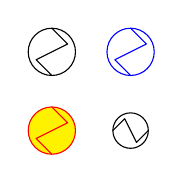
\begin{tikzpicture}
	\node[basic hx] at (0,0) {};
	\node[basic hx, draw=blue] at (1,0) {};
	\node[basic hx, draw=red, fill=yellow] at (0,-1) {};
	\node[basic hx, scale=0.75, rotate=90, anchor=center] at (1,-1) {};				
\end{tikzpicture}
		\end{lstlisting}
	\end{minipage}\hspace{0.25in}
	\begin{minipage}{1in}
		\begin{center}
			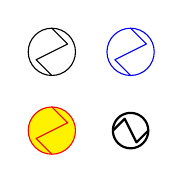
\begin{tikzpicture}
				\node[basic hx] at (0,0) {};
				\node[basic hx, draw=blue] at (1,0) {};
				\node[basic hx, draw=red, fill=yellow] at (0,-1) {};
				\node[basic hx, scale=0.75, rotate=90, thick] at (1,-1) {};				
			\end{tikzpicture}
		\end{center}
	\end{minipage}
\end{center}
Two additional PGF keys are available for some process units: |unit int| which modifies the interior contents of the process unit, and |unit ext| which modifies the exterior of the process unit.\footnote{A few other keys are available for drawing streams which are introduced later.} These keys can be used as
\begin{lstlisting}[numbers=none]
\node[<shape>, unit int=<intopt>, unit ext=<extopt>] {};
\end{lstlisting}
where |<intopt>| and |<extopt>| are interior and exterior options specific to the process unit. For most process units both keys can be used to combine effects. For example, the |basic hx| shape drawn above has keys |U tube| and |stems| which can be combined as follows:
\begin{center}
	\begin{minipage}{5in}
		\begin{lstlisting}
\begin{tikzpicture}
	\node[basic hx] at (0,0) {};
	\node[basic hx, unit ext=util] at (1,0) {};
	\node[basic hx, unit fill=U tube] at (0,-1) {};
	\node[basic hx, unit fill=U tube, unit ext=util] at (1,-1) {};		
\end{tikzpicture}
		\end{lstlisting}
	\end{minipage}\hspace{0.25in}
	\begin{minipage}{1in}
		\begin{center}
			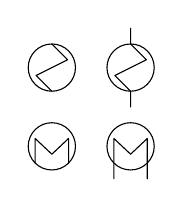
\begin{tikzpicture}
				\node[basic hx] at (0,0) {};
				\node[basic hx, unit ext=util] at (1,0) {};
				\node[basic hx, unit int=U tube] at (0,-1) {};
				\node[basic hx, unit int=U tube, unit ext=util] at (1,-1) {};		
			\end{tikzpicture}
		\end{center}
	\end{minipage}
\end{center}
However, unlike ``standard'' nodes \textit{the curly braces should always be empty}; that is, text cannot be directly included as part of the node (this prohibition includes keys like |label|). Annotations and labels of shapes from |pfdicons| must be included as separate nodes:
\begin{center}
	\begin{minipage}{5in}
		\begin{lstlisting}

\begin{tikzpicture}
	% No:
	% \node[basic hx] {H-101};
	
	% Yes:
	\node[basic hx] (g) {};
	\node[right] at (g.east) {H-101};				
\end{tikzpicture}
		\end{lstlisting}
	\end{minipage}\hspace{0.25in}
	\begin{minipage}{1in}
		\begin{center}
			
\begin{tikzpicture}
				% No:
				% \node[basic hx] {H-101};
				
				% Yes:
				\node[basic hx] (g) {};
				\node[right] at (g.east) {H-101};				
			\end{tikzpicture}
		\end{center}
	\end{minipage}
\end{center}

All process units have the standard cardinal and off-cardinal anchors which can be accessed using the standard \Tikz anchor notation such as |f.north| or |mycolumn.south east|. Some units have additional anchors on half-cardinal points (\textit{e.g.}, |north north east| or |east south east|) or special process unit features (\textit{e.g.}, |east jacket| or |actuator|). All compass anchors of custom shapes provided by the |pfdicons| package are \textbf{aliased with abbreviated versions} (\textit{e.g.}, |n| for |north|, |ene| for |east north east|) to allow for shortened code. Full anchor names can always be used to provide syntax consistency with core \Tikz.

\section{Process units}
\subsection{Reactors}
\subsubsection{Tank reactor}
\begin{lstlisting}[numbers=none]
\node[tank reactor] {};
\end{lstlisting}
\begin{figure}[h!]
	\centering
	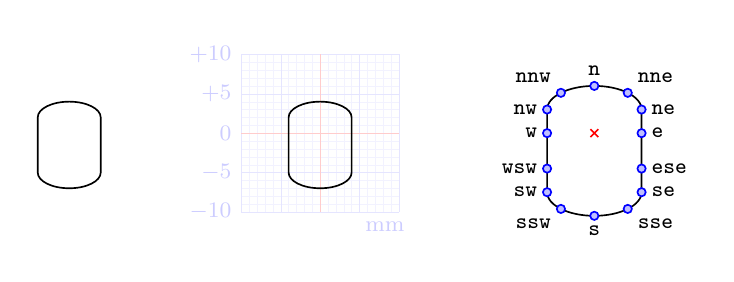
\begin{tikzpicture}[line width=0.6pt]
		\matrix[column sep=1cm, row sep=1cm, nodes={font=\footnotesize}]{%
		\node[tank reactor] {};	
		&
		\draw[help lines, blue!5, step=1mm, ultra thin] (-10mm, -10mm) grid (10mm, 10mm);
		\draw[help lines, blue!10, step=5mm, ultra thin] (-10mm, -10mm) grid (10mm, 10mm);
		\draw[red!20, thin] (-10mm,0mm) to (10mm, 0mm);
		\draw[red!20, thin] (0mm, -10mm) to (0mm, 10mm);
		\node[left] at (-10mm,0mm) {\color{blue!20}0};
		\node[left] at (-10mm,5mm) {\color{blue!20}$+5$};
		\node[left] at (-10mm,-5mm) {\color{blue!20}$-5$};
		\node[left] at (-10mm,10mm) {\color{blue!20}$+10$};
		\node[left] at (-10mm,-10mm){\color{blue!20}$-10$};
		\node[anchor=north east] at (12mm,-10mm) {\color{blue!20}mm}; 
		\node[tank reactor] {};
				&
		\node[tank reactor, scale=1.5] (f) {};
		
		\foreach \anchor/\pos in {
			n/above, 
			e/right, 
			w/left, 
			s/below}
		{\node[circle, draw, blue, fill=blue!25, inner sep=0pt, minimum size=3pt] at (f.\anchor) {};
			\node[\pos] at (f.\anchor) {\footnotesize\texttt{\textbf{\anchor}}};}
			
		\foreach \anchor/\pos in {
			ne/right, 
			nw/left, 
			se/right, 
			sw/left,
			nne/above right, 
			nnw/above left, 
			sse/below right, 
			ssw/below left,
			ese/right, 
			wsw/left}
		{\node[circle, draw, blue, fill=blue!25, inner sep=0pt, minimum size=3pt] at (f.\anchor) {};
		\node[\pos] at (f.\anchor) {\footnotesize\texttt{\anchor}};}

		\draw[shift=(f.center),red] plot[mark=x] coordinates{(0,0)};
		\\	
		};	
	\end{tikzpicture}
\end{figure}
The |tank reactor| shape provides a cylindrical tank reactor, also referred to as a stirred-tank reactor, continuous stirred-tank reactor (CSTRs), or autoclave. The |center| anchor is offset slightly to accommodate fill and interior options as described below. Several key modifiers are available:

\begin{center}
	\begin{longtable}{p{1.2in}p{2.5in}c}
		\caption{Key-value pairs for the \boldtt{tank reactor} shape.}\\
		\toprule
		\texttt{key=value} & Description & Example \\
		\midrule
		\endfirsthead
		
		\multicolumn{3}{c}{\tablename\ \thetable: Key-value pairs for the \boldtt{tank reactor} shape \textit{(cont'd)}} \\
		\midrule
		\endhead
		
		\bottomrule
		\endfoot
		
		\bottomrule
		\endlastfoot
		
		\texttt{unit int=stirred} & Adds a rounded stirrer with motor and 
		mixing blade. Three additional anchors are specific to this option: 
		\redtt{west motor}, \redtt{north motor}, and \redtt{east motor}. & 
		\adjustbox{valign=t}{
		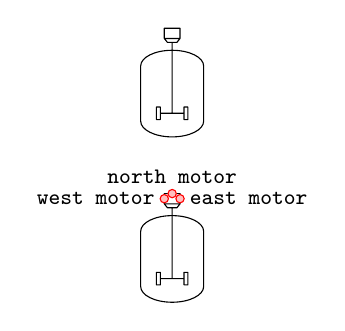
\begin{tikzpicture}
			\node[tank reactor, unit int=stirred] (f) {};
			\node[tank reactor, unit int=stirred, above=of f.north] {};
			\foreach \anchor/\pos in {
				west motor/left,
				north motor/above,
				east motor/right}
			{\node[circle, draw, red, fill=red!25, inner sep=0pt, minimum size=3pt] at (f.\anchor) {};
				\node[\pos] at (f.\anchor) {\footnotesize\texttt{\anchor}};}

		\end{tikzpicture}} \\ 
		& & \\
		
		\texttt{unit int=liquid} & Adds wavy lines from |west| to |east| to 
		indicate a liquid surface. & 
		\adjustbox{valign=t}{
			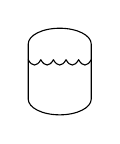
\begin{tikzpicture}
				\node[tank reactor, unit int=liquid] {};				
		\end{tikzpicture}} \\ 
		& & \\
		
		\texttt{unit int=stirred} \texttt{liquid} & A combination of |unit int=stirred| and |unit int=liquid|.
		& 
		\adjustbox{valign=t}{
			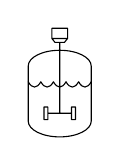
\begin{tikzpicture}
				\node[tank reactor, unit int=stirred liquid] {};				
		\end{tikzpicture}} \\ 
		& & \\
		
		\texttt{unit ext=lower} \texttt{jacket} & Adds a jacket around the lower portion of the reactor. Two additional anchors are specific to this option: \redtt{west jacket} and \redtt{east jacket}. & 
		\adjustbox{valign=t}{
			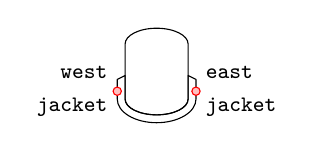
\begin{tikzpicture}
				\node[tank reactor, unit ext=lower jacket] (f) {};
				\foreach \anchor/\pos in {
					west jacket/left,
					east jacket/right}
				{\node[circle, draw, red, fill=red!25, inner sep=0pt, minimum size=3pt] at (f.\anchor) {};}
				
				\node[align=left, anchor=west] at (f.east jacket) {\footnotesize\texttt{east}\\ \footnotesize\texttt{jacket}};
				\node[align=right, anchor=east] at (f.west jacket) {\footnotesize\texttt{west}\\ \footnotesize\texttt{jacket}};
		\end{tikzpicture}} \\
		& & \\
		
		\texttt{unit ext=side} \texttt{jacket} & Adds a jacket around the side of the reactor. Several additional anchors available: \redtt{west jacket}, \redtt{north west jacket}, \redtt{south west jacket}, \redtt{east jacket}, \redtt{north east jacket}, and \redtt{south east jacket}. & 
		\adjustbox{valign=t}{
			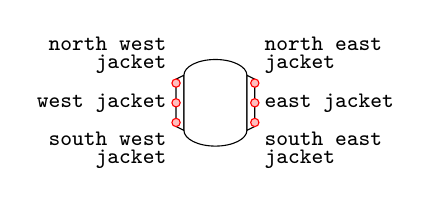
\begin{tikzpicture} [font=\footnotesize\ttfamily]
				\node[tank reactor, unit ext=side jacket] (f) {};
				\foreach \anchor in {
					west jacket,
					east jacket,
					north west jacket,
					north east jacket,
					south west jacket,
					south east jacket}
				{\node[circle, draw, red, fill=red!25, inner sep=0pt, minimum size=3pt] at (f.\anchor) {};}
				
				\node[align=left, anchor=west] at (f.east jacket) {east jacket};
				\node[align=left, anchor=south west] at (f.north east jacket) {north east\\[-3pt]jacket};
				\node[align=left, anchor=north west] at (f.south east jacket) {south east\\[-3pt]jacket};
				\node[align=right, anchor=east] at (f.west jacket) {west jacket};
				\node[align=right, anchor=south east] at (f.north west jacket) {north west\\[-3pt]jacket};
				\node[align=right, anchor=north east] at (f.south west jacket) {south west\\[-3pt]jacket};

		\end{tikzpicture}} \\
	\end{longtable}
\end{center}




\subsubsection{Tube reactor}
\begin{lstlisting}{numbers=none}
\node[tube reactor] {};
\end{lstlisting}
\begin{figure}[h!]
	\centering
	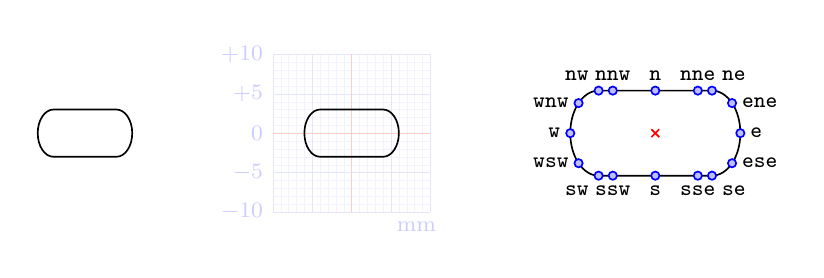
\begin{tikzpicture}[line width=0.6pt]
		\matrix[column sep=1cm, row sep=1cm, nodes={font=\footnotesize}]{%
			\node[tube reactor] {};	
			&
			\draw[help lines, blue!5, step=1mm, ultra thin] (-10mm, -10mm) grid (10mm, 10mm);
			\draw[help lines, blue!10, step=5mm, ultra thin] (-10mm, -10mm) grid (10mm, 10mm);
			\draw[red!20, thin] (-10mm,0mm) to (10mm, 0mm);
			\draw[red!20, thin] (0mm, -10mm) to (0mm, 10mm);
			\node[left] at (-10mm,0mm) {\color{blue!20}0};
			\node[left] at (-10mm,5mm) {\color{blue!20}$+5$};
			\node[left] at (-10mm,-5mm) {\color{blue!20}$-5$};
			\node[left] at (-10mm,10mm) {\color{blue!20}$+10$};
			\node[left] at (-10mm,-10mm){\color{blue!20}$-10$};
			\node[anchor=north east] at (12mm,-10mm) {\color{blue!20}mm}; 
			\node[tube reactor] {}; 
			&
			\node[tube reactor, scale=1.8] (f) {};
			
			\foreach \anchor/\pos in {
				n/above, 
				e/right, 
				w/left, 
				s/below}
			{\node[circle, draw, blue, fill=blue!25, inner sep=0pt, minimum size=3pt] at (f.\anchor) {};
				\node[\pos] at (f.\anchor) {\footnotesize\texttt{\textbf{\anchor}}};}
			
			\foreach \anchor/\pos in {
				ne/above right, 
				nw/above left, 
				se/below right, 
				sw/below left,
				nne/above, 
				nnw/above, 
				sse/below, 
				ssw/below,
				ese/right, 
				wsw/left,
				wnw/left,
				ene/right}
			{\node[circle, draw, blue, fill=blue!25, inner sep=0pt, minimum size=3pt] at (f.\anchor) {};
				\node[\pos] at (f.\anchor) {\footnotesize\texttt{\anchor}};}
			
			\draw[shift=(f.center),red] plot[mark=x] coordinates{(0,0)};
			\\	
		};	
	\end{tikzpicture}
\end{figure}
The |tube reactor| shape provides a horizontal cylinder with curved sides to be used for such reactors as plug flow reactors, packed bed reactors, fixed bed reactors, tubular reactors, and so forth. Several key-value pairs can be provided to indicate common fills and utility features:
\begin{center}
	\begin{longtable}{p{1.5in}p{3in}c}
		\caption{Key-value pairs for the \boldtt{tube reactor} shape.}\\
		\toprule
		\texttt{key=value} & Description & Example \\
		\midrule
		\endfirsthead
		
		\multicolumn{3}{c}{\tablename\ \thetable: Key-value pairs for the \boldtt{tube reactor} shape \textit{(cont'd)}} \\
		\midrule
		\endhead
		
		\bottomrule
		\endfoot
		
		\bottomrule
		\endlastfoot
		
		\texttt{unit int=packed} & Adds a cross representing a packed, dumped, or random fill within the reactor.  & 
		\adjustbox{valign=t}{
			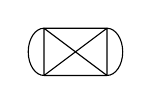
\begin{tikzpicture}
				\node[tube reactor, unit int=packed] {};
		\end{tikzpicture}} \\ 
		& & \\
		\texttt{unit int=fixed} & Adds angled lines representing a fixed bed.& 
		\adjustbox{valign=t}{
			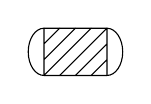
\begin{tikzpicture}
				\node[tube reactor, unit int=fixed] {};
		\end{tikzpicture}} \\
		& & \\
		\texttt{unit int=tubular} & Adds horizontal lines representing tubes for (\textit{e.g.}) shell-and-tube reactors, double-pipe reactors, and so forth.& 
		\adjustbox{valign=t}{
			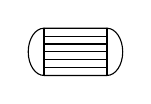
\begin{tikzpicture}
				\node[tube reactor, unit int=tubular] {};
		\end{tikzpicture}} \\
	
		& & \\
		\texttt{unit ext=cis shell} & Adds two shell-side stems, both on the north side with anchors \redtt{west shell} and \redtt{east shell}. Stems can be moved to the south side by rotating (|rotate=180|) or scaling (|yscale=-1|) the node. & 
		\adjustbox{valign=t}{
			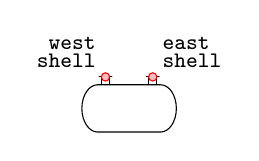
\begin{tikzpicture}[font=\footnotesize\ttfamily]
				\node[tube reactor, unit ext=cis shell] (f) {};
				\foreach \anchor in {west shell, east shell}
				{\node[circle, draw, red, fill=red!25, inner sep=0pt, minimum size=3pt] at (f.\anchor) {};}
				\node[align=right, anchor=south east] at (f.west shell) {west\\[-3pt]shell};
				\node[align=left, anchor=south west] at (f.east shell) {east\\[-3pt]shell};
		\end{tikzpicture}} \\
	
		& & \\ 
		\texttt{unit ext=trans shell} & Adds two shell-side stems, one on the north side and one on the south side, with anchors \redtt{north shell} and \redtt{south shell}. Stem locations can be swapped by scaling the node (|yscale=-1| or |xscale=-1|). & 
		\adjustbox{valign=t}{
			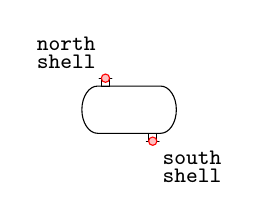
\begin{tikzpicture}[font=\footnotesize\ttfamily]
				\node[tube reactor, unit ext=trans shell] (f) {};
				\foreach \anchor in {north shell, south shell}
				{\node[circle, draw, red, fill=red!25, inner sep=0pt, minimum size=3pt] at (f.\anchor) {};}	
				\node[align=right, anchor=south east] at (f.north shell) {north\\[-3pt]shell};
				\node[align=left, anchor=north west] at (f.south shell) {south\\[-3pt]shell};
		\end{tikzpicture}} \\
	\end{longtable}
\end{center}






\subsection{Heat exchangers}
\subsubsection{Basic heat exchanger}
\begin{lstlisting}[numbers=none]
\node[basic hx] {};
\end{lstlisting}
\begin{figure}[h!]
	\centering
	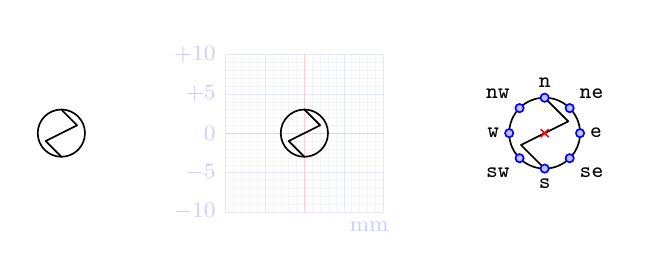
\begin{tikzpicture}[line width=0.6pt]
		\matrix[column sep=1cm, row sep=1cm, nodes={font=\footnotesize}]{%
			\node[basic hx] {};	
			&
			\draw[help lines, blue!5, step=1mm, ultra thin] (-10mm, -10mm) grid (10mm, 10mm);
			\draw[help lines, blue!10, step=5mm, ultra thin] (-10mm, -10mm) grid (10mm, 10mm);
			\draw[red!20, thin] (-10mm,0mm) to (10mm, 0mm);
			\draw[red!20, thin] (0mm, -10mm) to (0mm, 10mm);
			\node[left] at (-10mm,0mm) {\color{blue!20}0};
			\node[left] at (-10mm,5mm) {\color{blue!20}$+5$};
			\node[left] at (-10mm,-5mm) {\color{blue!20}$-5$};
			\node[left] at (-10mm,10mm) {\color{blue!20}$+10$};
			\node[left] at (-10mm,-10mm){\color{blue!20}$-10$};
			\node[anchor=north east] at (12mm,-10mm) {\color{blue!20}mm}; 
			\node[basic hx] {};
			&
			\node[basic hx, scale=1.5] (f) {};
			
			\foreach \anchor/\pos in {
				n/above, 
				e/right, 
				w/left, 
				s/below}
			{\node[circle, draw, blue, fill=blue!25, inner sep=0pt, minimum size=3pt] at (f.\anchor) {};
				\node[\pos] at (f.\anchor) {\footnotesize\texttt{\textbf{\anchor}}};}
			
			\foreach \anchor/\pos in {
				ne/above right, 
				nw/above left, 
				se/below right, 
				sw/below left}
			{\node[circle, draw, blue, fill=blue!25, inner sep=0pt, minimum size=3pt] at (f.\anchor) {};
				\node[\pos] at (f.\anchor) {\footnotesize\texttt{\anchor}};}
			
			\draw[shift=(f.center),red] plot[mark=x] coordinates{(0,0)};
			\\	
		};	
	\end{tikzpicture}
\end{figure}
The |basic hx| shape provides a circle with a jagged interior line and represents a generic heat exchange unit. Only the four cardinal and intercardinal anchors are used; the half-cardinals |nnw|, |nne|, |ssw|, and |sse| anchors are not used. Protrusions from the inner ``tube'' line can be added to provide additional indication of tube-side fluids, typically to indicate utility fluids (hence the |util| value). Additional anchors can be used to place labels at ends of the protrusions.
\begin{center}
	\begin{longtable}{p{1.5in}p{3in}c}
		\caption{Key-value pairs for the \boldtt{basic hx} shape.}\\
		\toprule
		\texttt{key=value} & Description & Example \\
		\midrule
		\endfirsthead
		
		\multicolumn{3}{c}{\tablename\ \thetable: Key-value pairs for the \boldtt{basic hx} shape \textit{(cont'd)}} \\
		\midrule
		\endhead
		
		\bottomrule
		\endfoot
		
		\bottomrule
		\endlastfoot
		
		\texttt{unit ext=util} & Adds protrusions from the inner tube, typically to indicate utility fluids. Additional anchors \redtt{south util} and \redtt{north util} are available at the terminals. & 
		\adjustbox{valign=t}{
			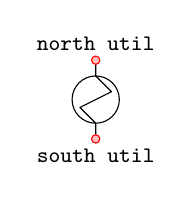
\begin{tikzpicture}
				\node[basic hx, unit ext=util] (f) {};
				\foreach \anchor/\pos in {
					north util/above,
					south util/below}
				{\node[circle, draw, red, fill=red!25, inner sep=0pt, minimum size=3pt] at (f.\anchor) {};
					\node[\pos] at (f.\anchor) {\footnotesize\texttt{\anchor}};}
		\end{tikzpicture}} \\ 
		& & \\
		\texttt{unit int=U tube} & Modifies interior to a generic U-tube orientation with both tube points on the same shell side. The |south west| and |south east| anchors are located at these tube points. & 
		\adjustbox{valign=t}{
			
\begin{tikzpicture}
				\node[basic hx, unit int=U tube] {};
		\end{tikzpicture}} \\
		& & \\
		\texttt{unit int=U tube,}\newline \texttt{unit ext=util} & Modifies interior to U-tube orientation and adds protrusions, typically to indicate utility fluids. Additional anchors \redtt{west util} and \redtt{east util} are available at the terminals. & 
		\adjustbox{valign=t}{
			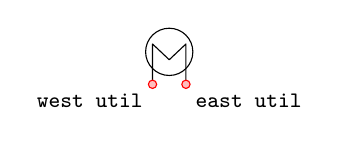
\begin{tikzpicture}
				\node[basic hx, unit int=U tube, unit ext=util] (f) {};
				\foreach \anchor/\pos in {
					west util/below left,
					east util/below right}
				{\node[circle, draw, red, fill=red!25, inner sep=0pt, minimum size=3pt] at (f.\anchor) {};
					\node[\pos] at (f.\anchor) {\footnotesize\texttt{\anchor}};}
		\end{tikzpicture}} \\
	\end{longtable}
\end{center}


\subsubsection{Shell and tube heat exchanger}
\begin{lstlisting}[numbers=none]
\node[shell and tube hx] {};
\end{lstlisting}
\begin{figure}[h!]
	\centering
	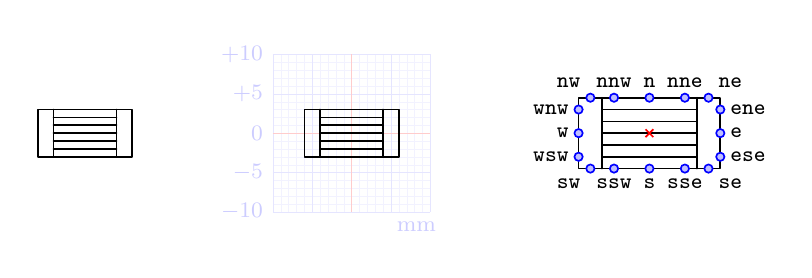
\begin{tikzpicture}[line width=0.6pt]
		\matrix[column sep=1cm, row sep=1cm, nodes={font=\footnotesize}]{%
			\node[shell and tube hx] (g) {};
			&
			\draw[help lines, blue!5, step=1mm, ultra thin] (-10mm, -10mm) grid (10mm, 10mm);
			\draw[help lines, blue!10, step=5mm, ultra thin] (-10mm, -10mm) grid (10mm, 10mm);
			\draw[red!20, thin] (-10mm,0mm) to (10mm, 0mm);
			\draw[red!20, thin] (0mm, -10mm) to (0mm, 10mm);
			\node[left] at (-10mm,0mm) {\color{blue!20}0};
			\node[left] at (-10mm,5mm) {\color{blue!20}$+5$};
			\node[left] at (-10mm,-5mm) {\color{blue!20}$-5$};
			\node[left] at (-10mm,10mm) {\color{blue!20}$+10$};
			\node[left] at (-10mm,-10mm){\color{blue!20}$-10$};
			\node[anchor=north east] at (12mm,-10mm) {\color{blue!20}mm}; 
			\node[shell and tube hx] {};
			&
			\node[shell and tube hx, scale=1.5] (f) {};
			
			\foreach \anchor/\pos in {
				n/above, 
				e/right, 
				w/left, 
				s/below}
			{\node[circle, draw, blue, fill=blue!25, inner sep=0pt, minimum size=3pt] at (f.\anchor) {};
				\node[\pos] at (f.\anchor) {\footnotesize\texttt{\textbf{\anchor}}};}
			
			\foreach \anchor/\pos in {
				ne/above right, 
				nw/above left, 
				se/below right, 
				sw/below left,
				nne/above, 
				nnw/above, 
				sse/below, 
				ssw/below,
				ese/right, 
				wsw/left,
				wnw/left,
				ene/right}
			{\node[circle, draw, blue, fill=blue!25, inner sep=0pt, minimum size=3pt] at (f.\anchor) {};
				\node[\pos] at (f.\anchor) {\footnotesize\texttt{\anchor}};}
			
			\draw[shift=(f.center),red] plot[mark=x] coordinates{(0,0)};
			\\	
		};	
	\end{tikzpicture}
\end{figure}
The |shell and tube hx| shape provides a rectangle with an inner set of horizontal lines representing a shell and tube heat exchanger. Keys can modify the appearance to provide shell-side stems or modify the tube ends to represent two-pass or four-pass arrangements.
\begin{center}
	\begin{longtable}{p{1.5in}p{3in}c}
		\caption{Key-value pairs for the \boldtt{shell and tube hx} shape.}\\
		\toprule
		\texttt{key=value} & Description & Example \\
		\midrule
		\endfirsthead
		
		\multicolumn{3}{c}{\tablename\ \thetable: Key-value pairs for the \boldtt{shell and tube hx} shape \textit{(cont'd)}} \\
		\midrule
		\endhead
		
		\bottomrule
		\endfoot
		
		\bottomrule
		\endlastfoot
		
		\texttt{unit int=two pass} & Adds a horizontal line on the west shell side to indicate a two-pass heat exchanger.& 
		\adjustbox{valign=t}{
			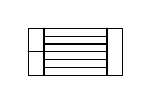
\begin{tikzpicture}
				\node[shell and tube hx, unit int=two pass] (f) {};
		\end{tikzpicture}} \\ 
		& & \\
		\texttt{unit int=four pass} & Adds two horizontal line on the west shell side and one on the east to indicate a four-pass heat exchanger.& 
		\adjustbox{valign=t}{
			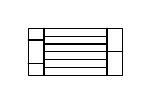
\begin{tikzpicture}
				\node[shell and tube hx, unit int=four pass] (f) {};
		\end{tikzpicture}} \\ 
		& & \\
		
		\texttt{unit ext=cis shell} & Adds two shell-side stems, both on the north side with anchors \redtt{west shell} and \redtt{east shell}. Stems can be moved to the south side by rotating (|rotate=180|) or scaling (|yscale=-1|) the node. & 
		\adjustbox{valign=t}{
			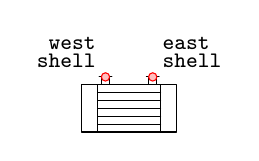
\begin{tikzpicture}[font=\footnotesize\ttfamily]
				\node[shell and tube hx, unit ext=cis shell] (f) {};
				\foreach \anchor in {west shell, east shell}
				{\node[circle, draw, red, fill=red!25, inner sep=0pt, minimum size=3pt] at (f.\anchor) {};}
				\node[align=right, anchor=south east] at (f.west shell) {west\\[-3pt]shell};
				\node[align=left, anchor=south west] at (f.east shell) {east\\[-3pt]shell};
		\end{tikzpicture}} \\
		
		& & \\ 
		\texttt{unit ext=trans shell} & Adds two shell-side stems, one on the north side and one on the south side, with anchors \redtt{north shell} and \redtt{south shell}. Stem locations can be swapped by scaling the node (|yscale=-1| or |xscale=-1|). & 
		\adjustbox{valign=t}{
			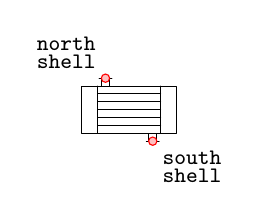
\begin{tikzpicture}[font=\footnotesize\ttfamily]
				\node[shell and tube hx, unit ext=trans shell] (f) {};
				\foreach \anchor in {north shell, south shell}
				{\node[circle, draw, red, fill=red!25, inner sep=0pt, minimum size=3pt] at (f.\anchor) {};}	
				\node[align=right, anchor=south east] at (f.north shell) {north\\[-3pt]shell};
				\node[align=left, anchor=north west] at (f.south shell) {south\\[-3pt]shell};
		\end{tikzpicture}} \\
	\end{longtable}
\end{center}



\subsubsection{Plate heat exchanger}
\begin{lstlisting}[numbers=none]
\node[plate hx] {};
\end{lstlisting}
\begin{figure}[h!]
	\centering
	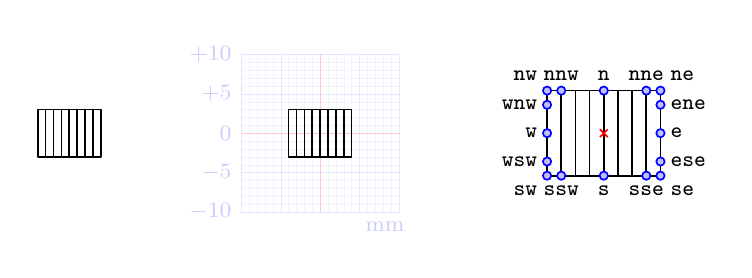
\begin{tikzpicture}[line width=0.6pt]
		\matrix[column sep=1cm, row sep=1cm, nodes={font=\footnotesize}]{%
			\node[plate hx] {};
			&
			\draw[help lines, blue!5, step=1mm, ultra thin] (-10mm, -10mm) grid (10mm, 10mm);
			\draw[help lines, blue!10, step=5mm, ultra thin] (-10mm, -10mm) grid (10mm, 10mm);
			\draw[red!20, thin] (-10mm,0mm) to (10mm, 0mm);
			\draw[red!20, thin] (0mm, -10mm) to (0mm, 10mm);
			\node[left] at (-10mm,0mm) {\color{blue!20}0};
			\node[left] at (-10mm,5mm) {\color{blue!20}$+5$};
			\node[left] at (-10mm,-5mm) {\color{blue!20}$-5$};
			\node[left] at (-10mm,10mm) {\color{blue!20}$+10$};
			\node[left] at (-10mm,-10mm){\color{blue!20}$-10$};
			\node[anchor=north east] at (12mm,-10mm) {\color{blue!20}mm}; 
			\node[plate hx] {};
			&
			\node[plate hx, scale=1.8] (f) {};
			
			\foreach \anchor/\pos in {
				n/above, 
				e/right, 
				w/left, 
				s/below}
			{\node[circle, draw, blue, fill=blue!25, inner sep=0pt, minimum size=3pt] at (f.\anchor) {};
				\node[\pos] at (f.\anchor) {\footnotesize\texttt{\textbf{\anchor}}};}
			
			\foreach \anchor/\pos in {
				ne/above right, 
				nw/above left, 
				se/below right, 
				sw/below left,
				nne/above, 
				nnw/above, 
				sse/below, 
				ssw/below,
				ese/right, 
				wsw/left,
				wnw/left,
				ene/right}
			{\node[circle, draw, blue, fill=blue!25, inner sep=0pt, minimum size=3pt] at (f.\anchor) {};
				\node[\pos] at (f.\anchor) {\footnotesize\texttt{\anchor}};}
			
			\draw[shift=(f.center),red] plot[mark=x] coordinates{(0,0)};
			\\	
		};	
	\end{tikzpicture}
\end{figure}
The |plate hx| shape provides a rectangle with an inner set of vertical lines representing a plate-and-frame heat exchanger. This unit has no |key=value| pairs for additional modification.


\subsubsection{Fired exchanger}
\begin{lstlisting}[numbers=none]
\node[fired hx] {};
\end{lstlisting}
\begin{figure}[h!]
	\centering
	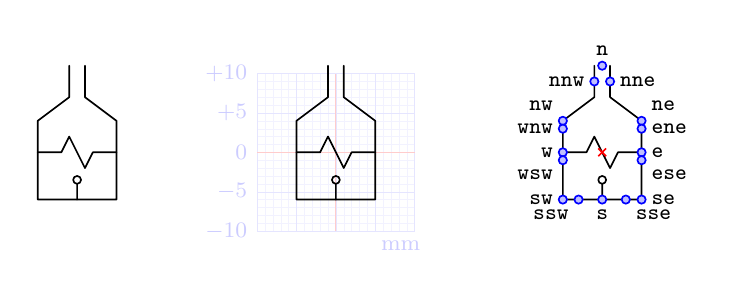
\begin{tikzpicture}[line width=0.6pt]
		\matrix[column sep=1cm, row sep=1cm, nodes={font=\footnotesize}]{%
			\node[fired hx] {};
			&
			\draw[help lines, blue!5, step=1mm, ultra thin] (-10mm, -10mm) grid (10mm, 10mm);
			\draw[help lines, blue!10, step=5mm, ultra thin] (-10mm, -10mm) grid (10mm, 10mm);
			\draw[red!20, thin] (-10mm,0mm) to (10mm, 0mm);
			\draw[red!20, thin] (0mm, -10mm) to (0mm, 10mm);
			\node[left] at (-10mm,0mm) {\color{blue!20}0};
			\node[left] at (-10mm,5mm) {\color{blue!20}$+5$};
			\node[left] at (-10mm,-5mm) {\color{blue!20}$-5$};
			\node[left] at (-10mm,10mm) {\color{blue!20}$+10$};
			\node[left] at (-10mm,-10mm){\color{blue!20}$-10$};
			\node[anchor=north east] at (12mm,-10mm) {\color{blue!20}mm}; 
			\node[fired hx] {};
			&
			\node[fired hx, scale=1] (f) {};
			
			\foreach \anchor/\pos in {
				n/above, 
				e/right, 
				w/left, 
				s/below}
			{\node[circle, draw, blue, fill=blue!25, inner sep=0pt, minimum size=3pt] at (f.\anchor) {};
				\node[\pos] at (f.\anchor) {\footnotesize\texttt{\textbf{\anchor}}};}
			
			\foreach \anchor/\pos in {
				ne/above right, 
				nw/above left, 
				se/right, 
				sw/left,
				nne/right, 
				nnw/left, 
				sse/below right, 
				ssw/below left,
				ese/below right, 
				wsw/below left,
				wnw/left,
				ene/right}
			{\node[circle, draw, blue, fill=blue!25, inner sep=0pt, minimum size=3pt] at (f.\anchor) {};
				\node[\pos] at (f.\anchor) {\footnotesize\texttt{\anchor}};}
			
			\draw[shift=(f.center),red] plot[mark=x] coordinates{(0,0)};
			\\	
		};	
	\end{tikzpicture}
\end{figure}
The |fired hx| shape provides a square unit with tapered chimney representing a fired heat exchanger. A horizontal through-line represents the process tube; a small circular icon at the bottom indicates the combustion region of the heat exchanger. The default number of process tubes is one (|unit int=single| or omitted) but additional process tubes can be added using the |unit int| key. Inlets and outlets will shift to correspond to half-cardinal anchors as shown below.
\begin{center}
	\begin{longtable}{p{1.5in}p{3in}c}
		\caption{Key-value pairs for the \boldtt{fired hx} shape.}\\
		\toprule
		\texttt{key=value} & Description & Example \\
		\midrule
		\endfirsthead
		
		\multicolumn{3}{c}{\tablename\ \thetable: Key-value pairs for the \boldtt{fired hx} shape \textit{(cont'd)}} \\
		\midrule
		\endhead
		
		\bottomrule
		\endfoot
		
		\bottomrule
		\endlastfoot
		
		\texttt{unit int=double} & Provides two tubes roughly corresponding to 
		the radiative and convective zones. & 
		\adjustbox{valign=t}{
			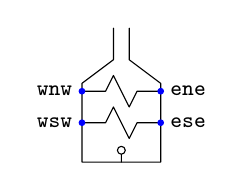
\begin{tikzpicture}
				\node[fired hx, unit int=double] (f) {};
				\foreach \anchor/\pos in {
					ese/right, 
					wsw/left,
					wnw/left,
					ene/right}
				{\node[circle, draw, blue, fill=blue, inner sep=0pt, minimum size=2pt] at (f.\anchor) {};
					\node[\pos] at (f.\anchor) {\footnotesize\texttt{\anchor}};}
		\end{tikzpicture}} \\ 
		& & \\
		\texttt{unit int=triple} & Provides three tubes roughly corresponding to a radiative zone and two convective zones. & 
		\adjustbox{valign=t}{
			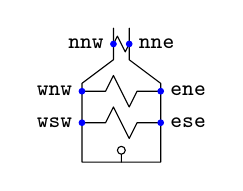
\begin{tikzpicture}
				\node[fired hx, unit int=triple] (f) {};
				\foreach \anchor/\pos in {
					nne/right, 
					nnw/left, 
					ese/right, 
					wsw/left,
					wnw/left,
					ene/right}
				{\node[circle, draw, blue, fill=blue, inner sep=0pt, minimum size=2pt] at (f.\anchor) {};
					\node[\pos] at (f.\anchor) {\footnotesize\texttt{\anchor}};}
		\end{tikzpicture}} \\
	\end{longtable}
\end{center}


\subsection{Separation units}
\subsubsection{Column}
\begin{lstlisting}[numbers=none]
\node[column] {};
\end{lstlisting}
\begin{figure}[h!]
	\centering
	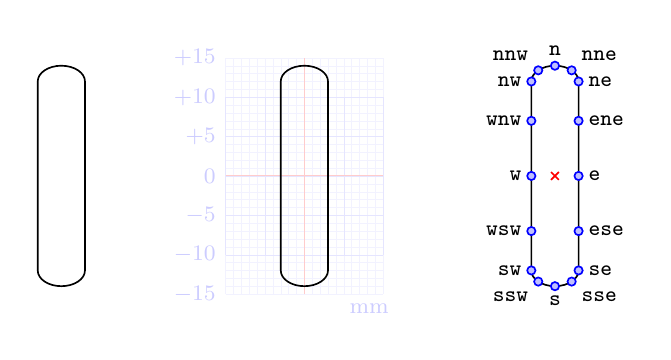
\begin{tikzpicture}[line width=0.6pt]
		\matrix[column sep=1cm, row sep=1cm, nodes={font=\footnotesize}]{%
			\node[column] {};	
			&
			\draw[help lines, blue!5, step=1mm, ultra thin] (-10mm, -15mm) grid (10mm, 15mm);
			\draw[help lines, blue!10, step=5mm, ultra thin] (-10mm, -10mm) grid (10mm, 10mm);
			\draw[red!20, thin] (-10mm,0mm) to (10mm, 0mm);
			\draw[red!20, thin] (0mm, -15mm) to (0mm, 15mm);
			\node[left] at (-10mm,0mm) {\color{blue!20}0};
			\node[left] at (-10mm,5mm) {\color{blue!20}$+5$};
			\node[left] at (-10mm,-5mm) {\color{blue!20}$-5$};
			\node[left] at (-10mm,10mm) {\color{blue!20}$+10$};
			\node[left] at (-10mm,-10mm){\color{blue!20}$-10$};
			\node[left] at (-10mm,15mm) {\color{blue!20}$+15$};
			\node[left] at (-10mm,-15mm){\color{blue!20}$-15$};
			\node[anchor=north east] at (12mm,-15mm) {\color{blue!20}mm}; 
			\node[column] {};
			&
			\node[column] (f) {};
			
			\foreach \anchor/\pos in {
				n/above, 
				e/right, 
				w/left, 
				s/below}
			{\node[circle, draw, blue, fill=blue!25, inner sep=0pt, minimum size=3pt] at (f.\anchor) {};
				\node[\pos] at (f.\anchor) {\footnotesize\texttt{\textbf{\anchor}}};}
			
			\foreach \anchor/\pos in {
				ne/right, 
				nw/left, 
				se/right, 
				sw/left,
				nne/above right, 
				nnw/above left, 
				sse/below right, 
				ssw/below left,
				ese/right, 
				wsw/left,
				wnw/left,
				ene/right}
			{\node[circle, draw, blue, fill=blue!25, inner sep=0pt, minimum size=3pt] at (f.\anchor) {};
				\node[\pos] at (f.\anchor) {\footnotesize\texttt{\anchor}};}
			
			\draw[shift=(f.center),red] plot[mark=x] coordinates{(0,0)};
			\\	
		};	
	\end{tikzpicture}
\end{figure}
The |column| shape provides a vertical, elongated cylinder as a generic separation column. The default fill is empty but several |key=value| pairs are provided to represent the most common separation units. Several additional anchors and keys are available based on these settings.

\begin{center}
	\begin{longtable}{p{1.75in}p{3in}c}
		\caption{Key-value pairs for the \boldtt{column} shape.}\\
		\toprule
		\texttt{key=value} & Description & Example \\
		\midrule
		\endfirsthead
			
		\multicolumn{3}{c}{\tablename\ \thetable: Key-value pairs for the \boldtt{column} shape \textit{(cont'd)}} \\
		\midrule
		\endhead
			
		\bottomrule
		\endfoot
			
		\bottomrule
		\endlastfoot
		
		\texttt{unit ext=simple hx} & Provides stylized representation of condenser and reboiler along with anchors \redtt{distillate} and \redtt{bottoms} for stream connections. These anchors always exist but coincide with |north east| and |south east| when the |simple hx| key is omitted.& 
		\adjustbox{valign=t}{
			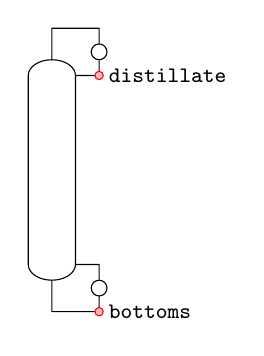
\begin{tikzpicture}
				\node[column, unit ext=simple hx] (f) {};
				\foreach \anchor/\pos in {
					distillate/right,
					bottoms/right}
				{\node[circle, draw, red, fill=red!25, inner sep=0pt, minimum size=3pt] at (f.\anchor) {};
					\node[\pos] at (f.\anchor) {\footnotesize\texttt{\anchor}};}
		\end{tikzpicture}} \\ 
	
		& & \\
		\texttt{unit int=tray}\newline \texttt{unit int=dashed tray} & Dashed, horizontal lines. Dashes will always have three segments and two openings.& 
		\adjustbox{valign=t}{
			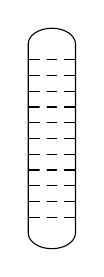
\begin{tikzpicture}
				\node[column, unit int=tray] (f) {};
		\end{tikzpicture}} \\
		& & \\
		
		\texttt{unit int=weir tray} & Solid, horizontal lines with small risers to 
		represent tray weirs.& 
		\adjustbox{valign=t}{
			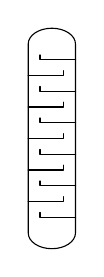
\begin{tikzpicture}
				\node[column, unit int=weir tray] (f) {};
		\end{tikzpicture}} \\
		& & \\
		
		\texttt{unit int=numbered tray}\newline\newline\hspace*{1em}\textit{associated keys:}\newline\hspace*{2em}\texttt{top tray=99}\newline\hspace*{2em}\texttt{feed tray=00}\newline\hspace*{2em}\texttt{bottom tray=22} & Dashed, horizontal lines at top, feed, and bottom trays. Associated keys |top tray|, |feed tray|, and |bottom tray| can be used to indicate tray numbers \textbf{if column is not transformed}. If column is transformed then associated keys can be omitted and anchors \redtt{feed tray}, \redtt{top tray}, and \redtt{bottom tray} used for placement of additional text nodes.& 
		\adjustbox{valign=t}{
			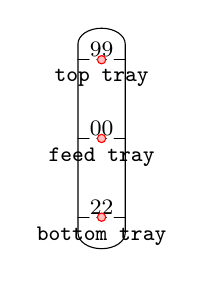
\begin{tikzpicture}
				\node[column, unit int=numbered tray, top tray=99, feed tray=00, 
				bottom tray=22] (f) {};
				\foreach \anchor/\pos in {
					top tray/below,
					feed tray/below,
					bottom tray/below}
				{\node[circle, draw, red, fill=red!25, inner sep=0pt, minimum size=3pt] at (f.\anchor) {};
					\node[\pos] at (f.\anchor) {\footnotesize\texttt{\anchor}};}
		\end{tikzpicture}} \\
		& & \\
		
		\texttt{unit int=packed} & Large cross symbol indicating random or dumped fill (packing).& 
		\adjustbox{valign=t}{
			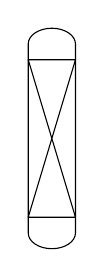
\begin{tikzpicture}
				\node[column, unit int=packed] (f) {};
		\end{tikzpicture}} \\
		& & \\
		
		\texttt{unit int=double packed} & Two sections of random or dumped fill (packing) separated by a small, central gap.& 
		\adjustbox{valign=t}{
			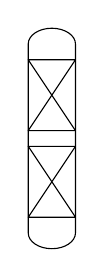
\begin{tikzpicture}
				\node[column, unit int=double packed] (f) {};
		\end{tikzpicture}} \\
\end{longtable}
\end{center}






\subsubsection{Vessel}
\begin{lstlisting}[numbers=none]
\node[vessel] {};
\end{lstlisting}
\begin{figure}[h!]
	\centering
	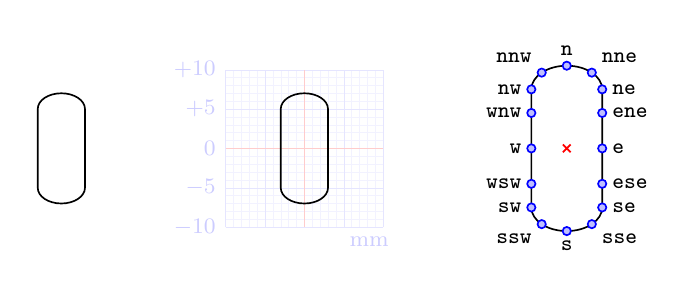
\begin{tikzpicture}[line width=0.6pt]
		\matrix[column sep=1cm, row sep=1cm, nodes={font=\footnotesize}]{%
			\node[vessel] {};	
			&
			\draw[help lines, blue!5, step=1mm, ultra thin] (-10mm, -10mm) grid (10mm, 10mm);
			\draw[help lines, blue!10, step=5mm, ultra thin] (-10mm, -10mm) grid (10mm, 10mm);
			\draw[red!20, thin] (-10mm,0mm) to (10mm, 0mm);
			\draw[red!20, thin] (0mm, -10mm) to (0mm, 10mm);
			\node[left] at (-10mm,0mm) {\color{blue!20}0};
			\node[left] at (-10mm,5mm) {\color{blue!20}$+5$};
			\node[left] at (-10mm,-5mm) {\color{blue!20}$-5$};
			\node[left] at (-10mm,10mm) {\color{blue!20}$+10$};
			\node[left] at (-10mm,-10mm){\color{blue!20}$-10$};
			\node[anchor=north east] at (12mm,-10mm) {\color{blue!20}mm}; 
			\node[vessel] {};
			&
			\node[vessel, scale=1.5] (f) {};
			
			\foreach \anchor/\pos in {
				n/above, 
				e/right, 
				w/left, 
				s/below}
			{\node[circle, draw, blue, fill=blue!25, inner sep=0pt, minimum size=3pt] at (f.\anchor) {};
				\node[\pos] at (f.\anchor) {\footnotesize\texttt{\textbf{\anchor}}};}
			
			\foreach \anchor/\pos in {
				ne/right, 
				nw/left, 
				se/right, 
				sw/left,
				nne/above right, 
				nnw/above left, 
				sse/below right, 
				ssw/below left,
				ese/right, 
				wsw/left,
				wnw/left,
				ene/right}
			{\node[circle, draw, blue, fill=blue!25, inner sep=0pt, minimum size=3pt] at (f.\anchor) {};
				\node[\pos] at (f.\anchor) {\footnotesize\texttt{\anchor}};}
			
			\draw[shift=(f.center),red] plot[mark=x] coordinates{(0,0)};
			\\	
		};	
	\end{tikzpicture}
\end{figure}
The |vessel| shape provides a vertical cylinder as a generic vessel. Such a vessel can be, for example, down-scaled and rotated 90${^\circ}$ can represent a product tank or a phase separator after a condenser. The default fill is empty but several |key=value| pairs are provided to represent two common vapor-liquid units as well as liquid accumulation tanks. Several additional anchors are available based on these settings.

\begin{center}
	\begin{longtable}{p{1.75in}p{3in}c}
		\caption{Key-value pairs for the \boldtt{vessel} shape.}\\
		\toprule
		\texttt{key=value} & Description & Example \\
		\midrule
		\endfirsthead
		
		\multicolumn{3}{c}{\tablename\ \thetable: Key-value pairs for the \boldtt{vessel} shape \textit{(cont'd)}} \\
		\midrule
		\endhead
		
		\bottomrule
		\endfoot
		
		\bottomrule
		\endlastfoot
		
		
		\texttt{unit int=liquid} & Adds wavy lines across the middle of the vessel to indicate a liquid level. & 
		\adjustbox{valign=t}{
			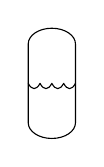
\begin{tikzpicture}
				\node[vessel, unit int=liquid] (f) {};
		\end{tikzpicture}} \\
		& & \\
		
		\texttt{unit int = liquid rotated} & Adds wavy lines down the center of the vessel to indicate a liquid level. This key is intended to be used with a rotated node such as
		\begin{lstlisting}[numbers=none]
\node[vessel, rotate=90, unit int=liquid rotated] {};
		\end{lstlisting}
		 & 
		\adjustbox{valign=t}{
			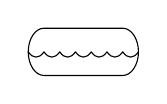
\begin{tikzpicture}
				\node[vessel, rotate=90, unit int=liquid rotated] (f) {};
		\end{tikzpicture}} \\
		& & \\
		
		\texttt{unit int=phase sep} & Adds a knock-down element near the |west| anchor and a dashed, horizontal line near the top of the vessel to indicate a demister pad. & 
		\adjustbox{valign=t}{
			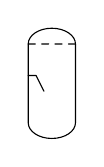
\begin{tikzpicture}
				\node[vessel, unit int=phase sep] (f) {};
		\end{tikzpicture}} \\
		& & \\
		
		\texttt{unit ext=simple hx} & Adds a simplified heat transfer element to the bottom portion of the vessel. Two additional anchors, \redtt{north hx} and \redtt{south hx}, are located at the exterior points of the heat exchanger tubes. & 
		\adjustbox{valign=t}{
			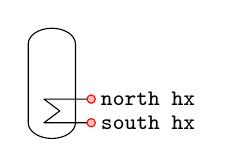
\begin{tikzpicture}
				\node[vessel, unit ext=simple hx] (f) {};
				\foreach \anchor/\pos in {
					north hx/right,
					south hx/right}
				{\node[circle, draw, red, fill=red!25, inner sep=0pt, minimum size=3pt] at (f.\anchor) {};
					\node[\pos] at (f.\anchor) {\footnotesize\texttt{\anchor}};}
		\end{tikzpicture}} \\ 
		
		& & \\
	\end{longtable}
\end{center}




\subsection{Fluid transport}
\subsubsection{Centrifugal pump}
\begin{lstlisting}[numbers=none]
\node[centrifugal pump] {};
\end{lstlisting}
\begin{figure}[h!]
	\centering
	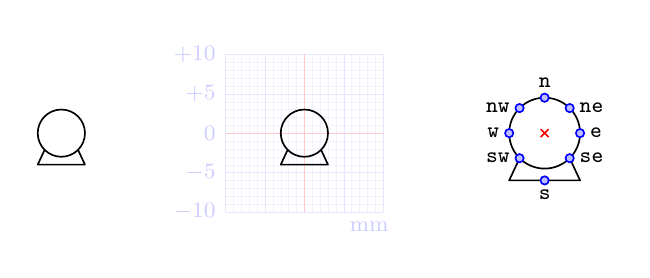
\begin{tikzpicture}[line width=0.6pt]
		\matrix[column sep=1cm, row sep=1cm, nodes={font=\footnotesize}]{%
			\node[centrifugal pump] {};	
			&
			\draw[help lines, blue!5, step=1mm, ultra thin] (-10mm, -10mm) grid (10mm, 10mm);
			\draw[help lines, blue!10, step=5mm, ultra thin] (-10mm, -10mm) grid (10mm, 10mm);
			\draw[red!20, thin] (-10mm,0mm) to (10mm, 0mm);
			\draw[red!20, thin] (0mm, -10mm) to (0mm, 10mm);
			\node[left] at (-10mm,0mm) {\color{blue!20}0};
			\node[left] at (-10mm,5mm) {\color{blue!20}$+5$};
			\node[left] at (-10mm,-5mm) {\color{blue!20}$-5$};
			\node[left] at (-10mm,10mm) {\color{blue!20}$+10$};
			\node[left] at (-10mm,-10mm){\color{blue!20}$-10$};
			\node[anchor=north east] at (12mm,-10mm) {\color{blue!20}mm}; 
			\node[centrifugal pump] {};
			&
			\node[centrifugal pump, scale=1.5] (f) {};
			
			\foreach \anchor/\pos in {
				n/above, 
				e/right, 
				w/left, 
				s/below}
			{\node[circle, draw, blue, fill=blue!25, inner sep=0pt, minimum size=3pt] at (f.\anchor) {};
				\node[\pos] at (f.\anchor) {\footnotesize\texttt{\textbf{\anchor}}};}
			
			\foreach \anchor/\pos in {
				ne/right, 
				nw/left, 
				se/right, 
				sw/left}
			{\node[circle, draw, blue, fill=blue!25, inner sep=0pt, minimum size=3pt] at (f.\anchor) {};
				\node[\pos] at (f.\anchor) {\footnotesize\texttt{\anchor}};}
			
			\draw[shift=(f.center),red] plot[mark=x] coordinates{(0,0)};
			\\	
		};	
	\end{tikzpicture}
\end{figure}

\newpage
The |centrifugal pump| shape provides a circular element with a triangular base to represent a centrifugal pump. An additional half-circle can be added using the |unit int| key to indicate the pump inlet and a rectangular outlet direction can be added using the |unit ext| key.

\begin{center}
	\begin{longtable}{p{1.75in}p{3in}c}
		\caption{Key-value pairs for the \boldtt{centrifugal pump} shape.}\\
		\toprule
		\texttt{key=value} & Description & Example \\
		\midrule
		\endfirsthead
		
		\multicolumn{3}{c}{\tablename\ \thetable: Key-value pairs for the \boldtt{centrifugal pump} shape \textit{(cont'd)}} \\
		\midrule
		\endhead
		
		\bottomrule
		\endfoot
		
		\bottomrule
		\endlastfoot
		
		\texttt{unit int=inlet west} & Adds a half-circle around the |center| anchor to accept an inlet stream to enter from the west. & 
		\adjustbox{valign=t}{
			
\begin{tikzpicture}
				\node[centrifugal pump, unit int=inlet west] (f) {};
		\end{tikzpicture}} \\
		& & \\
		
		\texttt{unit int=inlet east} & Adds a half-circle around the |center| anchor to accept an inlet stream to enter from the east. & 
		\adjustbox{valign=t}{
			
\begin{tikzpicture}
				\node[centrifugal pump, unit int=inlet east] (f) {};
		\end{tikzpicture}} \\
		& & \\
		
		\texttt{unit int=inlet north} & Adds a half-circle around the |center| anchor to accept an inlet stream to enter from the north. & 
		\adjustbox{valign=t}{
			
\begin{tikzpicture}
				\node[centrifugal pump, unit int=inlet north] (f) {};
		\end{tikzpicture}} \\
		& & \\
		
		\texttt{unit int=inlet south} & Adds a half-circle around the |center| anchor to accept an inlet stream to enter from the south. Note that there is no means of removing the triangular base; such an inlet stream should be drawn as going through the base. & 
		\adjustbox{valign=t}{
			
\begin{tikzpicture}
				\node[centrifugal pump, unit int=inlet south] (f) {};
		\end{tikzpicture}} \\
		& & \\
		
		\texttt{unit ext=outlet east} & Adds a rectangular protrusion facing east to represent an outlet. Also adds the \redtt{outlet} anchor in the center of the outlet box. & 
		\adjustbox{valign=t}{
			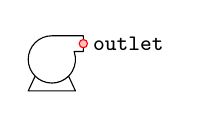
\begin{tikzpicture}
				\node[centrifugal pump, unit ext=outlet east] (f) {};
				\node[circle, draw, red, fill=red!25, inner sep=0pt, minimum size=3pt] at (f.outlet) {};
				\node[right] at (f.outlet) {\footnotesize\texttt{outlet}};
		\end{tikzpicture}} \\
		
		& & \\
		\texttt{unit ext=outlet west} & Adds a rectangular protrusion facing west to represent an outlet. Also adds the \redtt{outlet} anchor in the center of the outlet box. & 
		\adjustbox{valign=t}{
			\begin{tikzpicture}
				\node[centrifugal pump, unit ext=outlet west] (f) {};
				\node[circle, draw, red, fill=red!25, inner sep=0pt, minimum size=3pt] at (f.outlet) {};
				\node[left] at (f.outlet) {\footnotesize\texttt{outlet}};
		\end{tikzpicture}} \\
		
		& & \\
		\texttt{unit ext=outlet north east} & Adds a rectangular protrusion facing north on the east side of the pump to represent an outlet. Also adds the \redtt{outlet} anchor in the center of the outlet box. & 
		\adjustbox{valign=t}{
			\begin{tikzpicture}
				\node[centrifugal pump, unit ext=outlet north east] (f) {};
				\node[circle, draw, red, fill=red!25, inner sep=0pt, minimum size=3pt] at (f.outlet) {};
				\node[above] at (f.outlet) {\footnotesize\texttt{outlet}};
		\end{tikzpicture}} \\
		
		& & \\
		\texttt{unit ext=outlet north west} & Adds a rectangular protrusion facing north on the west side of the pump  to represent an outlet. Also adds the \redtt{outlet} anchor in the center of the outlet box. & 
		\adjustbox{valign=t}{
			\begin{tikzpicture}
				\node[centrifugal pump, unit ext=outlet north west] (f) {};
				\node[circle, draw, red, fill=red!25, inner sep=0pt, minimum size=3pt] at (f.outlet) {};
				\node[above] at (f.outlet) {\footnotesize\texttt{outlet}};
		\end{tikzpicture}} \\
		& & \\

	\end{longtable}
\end{center}




\subsubsection{Reciprocating pump}
\begin{lstlisting}[numbers=none]
\node[reciprocating pump] {};
\end{lstlisting}
\begin{figure}[h!]
	\centering
	\begin{tikzpicture}[line width=0.6pt]
		\matrix[column sep=1cm, row sep=1cm, nodes={font=\footnotesize}]{%
			\node[reciprocating pump] {};	
			&
			\draw[help lines, blue!5, step=1mm, ultra thin] (-10mm, -10mm) grid (10mm, 10mm);
			\draw[help lines, blue!10, step=5mm, ultra thin] (-10mm, -10mm) grid (10mm, 10mm);
			\draw[red!20, thin] (-10mm,0mm) to (10mm, 0mm);
			\draw[red!20, thin] (0mm, -10mm) to (0mm, 10mm);
			\node[left] at (-10mm,0mm) {\color{blue!20}0};
			\node[left] at (-10mm,5mm) {\color{blue!20}$+5$};
			\node[left] at (-10mm,-5mm) {\color{blue!20}$-5$};
			\node[left] at (-10mm,10mm) {\color{blue!20}$+10$};
			\node[left] at (-10mm,-10mm){\color{blue!20}$-10$};
			\node[anchor=north east] at (12mm,-10mm) {\color{blue!20}mm}; 
			\node[reciprocating pump] {};
			&
			\node[reciprocating pump, scale=1] (f) {};
			
			\foreach \anchor/\pos in {
				n/above, 
				e/right, 
				w/left, 
				s/below}
			{\node[circle, draw, blue, fill=blue!25, inner sep=0pt, minimum size=3pt] at (f.\anchor) {};
				\node[\pos] at (f.\anchor) {\footnotesize\texttt{\textbf{\anchor}}};}
			
			\foreach \anchor/\pos in {
				ne/right, 
				nw/left, 
				se/right, 
				sw/left}
			{\node[circle, draw, blue, fill=blue!25, inner sep=0pt, minimum size=3pt] at (f.\anchor) {};
				\node[\pos] at (f.\anchor) {\footnotesize\texttt{\anchor}};}
			
			\draw[shift=(f.center),red] plot[mark=x] coordinates{(0,0)};
			\\	
		};	
	\end{tikzpicture}
\end{figure}
The |reciprocating pump| shape provides two square elements--a pump head and motor--connected by a simple shaft. Most anchors are placed relative to the pump head. This unit has no |key=value| pairs for additional modification.


\subsubsection{Compressor}
\begin{lstlisting}[numbers=none]
\node[compressor] {};
\end{lstlisting}
\begin{figure}[h!]
	\centering
	\begin{tikzpicture}[line width=0.6pt]
		\matrix[column sep=1cm, row sep=1cm, nodes={font=\footnotesize}]{%
			\node[compressor] {};	
			&
			\draw[help lines, blue!5, step=1mm, ultra thin] (-10mm, -10mm) grid (10mm, 10mm);
			\draw[help lines, blue!10, step=5mm, ultra thin] (-10mm, -10mm) grid (10mm, 10mm);
			\draw[red!20, thin] (-10mm,0mm) to (10mm, 0mm);
			\draw[red!20, thin] (0mm, -10mm) to (0mm, 10mm);
			\node[left] at (-10mm,0mm) {\color{blue!20}0};
			\node[left] at (-10mm,5mm) {\color{blue!20}$+5$};
			\node[left] at (-10mm,-5mm) {\color{blue!20}$-5$};
			\node[left] at (-10mm,10mm) {\color{blue!20}$+10$};
			\node[left] at (-10mm,-10mm){\color{blue!20}$-10$};
			\node[anchor=north east] at (12mm,-10mm) {\color{blue!20}mm}; 
			\node[compressor] {};
			&
			\node[compressor, scale=2.5] (f) {};
			
			\foreach \anchor/\pos in {
				n/above, 
				e/right, 
				w/left, 
				s/below}
			{\node[circle, draw, blue, fill=blue!25, inner sep=0pt, minimum size=3pt] at (f.\anchor) {};
				\node[\pos] at (f.\anchor) {\footnotesize\texttt{\textbf{\anchor}}};}
			
			\foreach \anchor/\pos in {
				ne/above right, 
				nw/left, 
				se/below right, 
				sw/left,
				nne/above, 
				nnw/above, 
				sse/below, 
				ssw/below,
				ese/right, 
				wsw/left,
				wnw/left,
				ene/right}
			{\node[circle, draw, blue, fill=blue!25, inner sep=0pt, minimum size=3pt] at (f.\anchor) {};
				\node[\pos] at (f.\anchor) {\footnotesize\texttt{\anchor}};}
			
			\draw[shift=(f.center),red] plot[mark=x] coordinates{(0,0)};
			\\	
		};	
	\end{tikzpicture}
\end{figure}
The |compressor| shape provides a quadrilateral to represent a gas-phase compressor. This unit has no |key=value| pairs for additional modification. If mirrored along the $x$-axis (\textit{e.g.}, by using something like |xscale=-1| or |rotate=90|) then the |compressor| shape is identical to the |turbine| shape but with different anchor points.



\subsubsection{Turbine}
\begin{lstlisting}[numbers=none]
\node[turbine] {};
\end{lstlisting}
\begin{figure}[h!]
	\centering
	\begin{tikzpicture}[line width=0.6pt]
		\matrix[column sep=1cm, row sep=1cm, nodes={font=\footnotesize}]{%
			\node[turbine] {};	
			&
			\draw[help lines, blue!5, step=1mm, ultra thin] (-10mm, -10mm) grid (10mm, 10mm);
			\draw[help lines, blue!10, step=5mm, ultra thin] (-10mm, -10mm) grid (10mm, 10mm);
			\draw[red!20, thin] (-10mm,0mm) to (10mm, 0mm);
			\draw[red!20, thin] (0mm, -10mm) to (0mm, 10mm);
			\node[left] at (-10mm,0mm) {\color{blue!20}0};
			\node[left] at (-10mm,5mm) {\color{blue!20}$+5$};
			\node[left] at (-10mm,-5mm) {\color{blue!20}$-5$};
			\node[left] at (-10mm,10mm) {\color{blue!20}$+10$};
			\node[left] at (-10mm,-10mm){\color{blue!20}$-10$};
			\node[anchor=north east] at (12mm,-10mm) {\color{blue!20}mm}; 
			\node[turbine] {};
			&
			\node[turbine, scale=2.5] (f) {};
			
			\foreach \anchor/\pos in {
				n/above, 
				e/right, 
				w/left, 
				s/below}
			{\node[circle, draw, blue, fill=blue!25, inner sep=0pt, minimum size=3pt] at (f.\anchor) {};
				\node[\pos] at (f.\anchor) {\footnotesize\texttt{\textbf{\anchor}}};}
			
			\foreach \anchor/\pos in {
				ne/right, 
				nw/above left, 
				se/right, 
				sw/below left,
				nne/above, 
				nnw/above, 
				sse/below, 
				ssw/below,
				ese/right, 
				wsw/left,
				wnw/left,
				ene/right}
			{\node[circle, draw, blue, fill=blue!25, inner sep=0pt, minimum size=3pt] at (f.\anchor) {};
				\node[\pos] at (f.\anchor) {\footnotesize\texttt{\anchor}};}
			
			\draw[shift=(f.center),red] plot[mark=x] coordinates{(0,0)};
			\\	
		};	
	\end{tikzpicture}
\end{figure}
The |turbine| shape provides a quadrilateral to represent a gas-phase turbine. This unit has no |key=value| pairs for additional modification. If mirrored along the $x$-axis (\textit{e.g.}, by using something like |xscale=-1| or |rotate=90|) then the |turbine| shape is identical to the |compressor| shape but with different anchor points.





\section{Streams}


\subsection{Feed terminal}
\begin{lstlisting}[numbers=none]
\node[feed] {};
\end{lstlisting}
\begin{figure}[h!]
	\centering
	\begin{tikzpicture}[line width=0.6pt]
		\matrix[column sep=1cm, row sep=1cm, nodes={font=\footnotesize}]{%
			\node[feed] {};	
			&
			\draw[help lines, blue!5, step=1mm, ultra thin] (-10mm, -10mm) grid (10mm, 10mm);
			\draw[help lines, blue!10, step=5mm, ultra thin] (-10mm, -10mm) grid (10mm, 10mm);
			\draw[red!20, thin] (-10mm,0mm) to (10mm, 0mm);
			\draw[red!20, thin] (0mm, -10mm) to (0mm, 10mm);
			\node[left] at (-10mm,0mm) {\color{blue!20}0};
			\node[left] at (-10mm,5mm) {\color{blue!20}$+5$};
			\node[left] at (-10mm,-5mm) {\color{blue!20}$-5$};
			\node[left] at (-10mm,10mm) {\color{blue!20}$+10$};
			\node[left] at (-10mm,-10mm){\color{blue!20}$-10$};
			\node[anchor=north east] at (12mm,-10mm) {\color{blue!20}mm}; 
			\node[feed] {};
			&
			\node[feed, scale=2] (f) {};
			
			\foreach \anchor/\pos in {
				n/above, 
				w/left, 
				s/below}
			{\node[circle, draw, blue, fill=blue!25, inner sep=0pt, minimum size=3pt] at (f.\anchor) {};
				\node[\pos] at (f.\anchor) {\footnotesize\texttt{\textbf{\anchor}}};}
			
			\node[circle, draw, red, fill=red!25, inner sep=0pt, minimum size=3pt] at (f.stream) {};
			\node[right] at (f.stream) {\footnotesize\texttt{\textbf{e}} \textit{or} \redtt{stream}};
			
			\foreach \anchor/\pos in {
				ne/above right, 
				nw/above left, 
				se/below right, 
				sw/below left}
			{\node[circle, draw, blue, fill=blue!25, inner sep=0pt, minimum size=3pt] at (f.\anchor) {};
				\node[\pos] at (f.\anchor) {\footnotesize\texttt{\anchor}};}
			
			\draw[shift=(f.center),red] plot[mark=x] coordinates{(0,0)};
			\\	
		};	
	\end{tikzpicture}
\end{figure}
The |feed| shape provides a half-filled circle representing a process feed point. The special anchor \redtt{stream} corresponds to the |east| anchor and is provided as an optional method to define stream starting points. This unit has no |key=value| pairs for additional modification.




\subsection{Product terminal}
\begin{lstlisting}[numbers=none]
\node[product] {};
\end{lstlisting}
\begin{figure}[h!]
	\centering
	\begin{tikzpicture}[line width=0.6pt]
		\matrix[column sep=1cm, row sep=1cm, nodes={font=\footnotesize}]{%
			\node[product] {};	
			&
			\draw[help lines, blue!5, step=1mm, ultra thin] (-10mm, -10mm) grid (10mm, 10mm);
			\draw[help lines, blue!10, step=5mm, ultra thin] (-10mm, -10mm) grid (10mm, 10mm);
			\draw[red!20, thin] (-10mm,0mm) to (10mm, 0mm);
			\draw[red!20, thin] (0mm, -10mm) to (0mm, 10mm);
			\node[left] at (-10mm,0mm) {\color{blue!20}0};
			\node[left] at (-10mm,5mm) {\color{blue!20}$+5$};
			\node[left] at (-10mm,-5mm) {\color{blue!20}$-5$};
			\node[left] at (-10mm,10mm) {\color{blue!20}$+10$};
			\node[left] at (-10mm,-10mm){\color{blue!20}$-10$};
			\node[anchor=north east] at (12mm,-10mm) {\color{blue!20}mm}; 
			\node[product] {};
			&
			\node[product, scale=2] (f) {};
			
			\foreach \anchor/\pos in {
				n/above, 
				e/right, 
				s/below}
			{\node[circle, draw, blue, fill=blue!25, inner sep=0pt, minimum size=3pt] at (f.\anchor) {};
				\node[\pos] at (f.\anchor) {\footnotesize\texttt{\textbf{\anchor}}};}
			
			\node[circle, draw, red, fill=red!25, inner sep=0pt, minimum size=3pt] at (f.stream) {};
			\node[left] at (f.stream) {\footnotesize \redtt{stream} \textit{or} \boldtt{w}};
			
			\foreach \anchor/\pos in {
				ne/above right, 
				nw/above left, 
				se/below right, 
				sw/below left}
			{\node[circle, draw, blue, fill=blue!25, inner sep=0pt, minimum size=3pt] at (f.\anchor) {};
				\node[\pos] at (f.\anchor) {\footnotesize\texttt{\anchor}};}
			
			\draw[shift=(f.center),red] plot[mark=x] coordinates{(0,0)};
			\\	
		};	
	\end{tikzpicture}
\end{figure}
The |product| shape provides a half-filled circle representing a process product point. The special anchor \redtt{stream} corresponds to the |west| anchor and is provided as an optional method to define stream ending points. This unit has no |key=value| pairs for additional modification.



\subsection{Stream numbers}
\begin{lstlisting}[numbers=none]
\node[sid] {99};
\end{lstlisting}
\begin{figure}[h!]
	\centering
	\begin{tikzpicture}[line width=0.6pt]
		\matrix[column sep=1cm, row sep=1cm, nodes={font=\footnotesize}]{%
			\node[sid] {99};	
			&
			\draw[help lines, blue!5, step=1mm, ultra thin] (-10mm, -10mm) grid (10mm, 10mm);
			\draw[help lines, blue!10, step=5mm, ultra thin] (-10mm, -10mm) grid (10mm, 10mm);
			\draw[red!20, thin] (-10mm,0mm) to (10mm, 0mm);
			\draw[red!20, thin] (0mm, -10mm) to (0mm, 10mm);
			\node[left] at (-10mm,0mm) {\color{blue!20}0};
			\node[left] at (-10mm,5mm) {\color{blue!20}$+5$};
			\node[left] at (-10mm,-5mm) {\color{blue!20}$-5$};
			\node[left] at (-10mm,10mm) {\color{blue!20}$+10$};
			\node[left] at (-10mm,-10mm){\color{blue!20}$-10$};
			\node[anchor=north east] at (12mm,-10mm) {\color{blue!20}mm}; 
			\node[sid] {99};
			&
			\node[sid, scale=2] (f) {99};		
			\foreach \anchor/\pos in {
				north/above, 
				east/right, 
				west/left, 
				south/below}
			{\node[circle, draw, blue, fill=blue!25, inner sep=0pt, minimum size=3pt] at (f.\anchor) {};
				\node[\pos] at (f.\anchor) {\footnotesize\texttt{\textbf{\anchor}}};}
			
			\foreach \anchor/\pos in {
				north east/above right, 
				north west/above left, 
				south east/below right, 
				south west/below left}
			{\node[circle, draw, blue, fill=blue!25, inner sep=0pt, minimum size=3pt] at (f.\anchor) {};
				\node[\pos] at (f.\anchor) {\footnotesize\texttt{\anchor}};}
			
			\draw[shift=(f.center),red] plot[mark=x] coordinates{(0,0)};
			\\	
		};	
	\end{tikzpicture}
\end{figure}
The |sid| (read ``ess eye dee'' for ``stream identification'') shape provides a modified |diamond| shape from the |shapes| library for the purpose of labeling streams. The anchors \textbf{are not aliased} with their abbreviations because \textit{(a)} this is not a custom shape of the |pfdicons| package and \textit{(b)} the |sid| shape is typically used within a line (stream) without accessing its anchors. The fill of |sid| is white which allows it to be conveniently placed within a stream-drawing command such as
\begin{center}
	\begin{minipage}{5in}
		\begin{lstlisting}
\begin{tikzpicture}
	\draw[->] (0,0) -- node[sid] {00} (2,0);
\end{tikzpicture}
		\end{lstlisting}
	\end{minipage}\hspace{0.25in}
	\begin{minipage}{1in}
		\begin{center}
			\begin{tikzpicture}
				\draw[->] (0,0) -- node[sid] {00} (2,0);
			\end{tikzpicture}
		\end{center}
	\end{minipage}
\end{center}
The |sid| shape has no |key=value| pairs to modify its appearance but you can modify the appearance by redefining its |tikzstyle|, which by default is
\begin{lstlisting}[numbers=none]
\tikzstyle{sid} = [diamond, draw, solid, fill=white, text badly centered, inner sep=1pt, font=\footnotesize]
\end{lstlisting}
Modifications to this definition can occur either in the preamble (to affect all drawings) or within the document (to affect individual drawings or lines). For example, if you'd like to use circular identifiers with a blue fill and more space around bigger numbers then you could do something like this:
\begin{center}
	\begin{minipage}{5in}
		\begin{lstlisting}
\begin{tikzpicture}
	\draw[->] (0,0) -- node[sid] {1} (2,0);
	
	\tikzstyle{sid} = [circle, draw, solid, fill=blue!15, text badly centered, inner sep=3pt, font=\tiny]
	
	\draw[->] (0,-1) -- node[sid] {2} (2,-1);
	
	\draw[->] (0,-2) -- node[sid] {3} (2,-2);
\end{tikzpicture}
		\end{lstlisting}
	\end{minipage}\hspace{0.25in}
	\begin{minipage}{1in}
		\begin{center}
			\begin{tikzpicture}
				\draw[->] (0,0) -- node[sid] {1} (2,0);
				
				\tikzstyle{sid} = [circle, draw, solid, 
				fill=blue!15, text badly centered,
				inner sep=3pt, font=\tiny]
				
				\draw[->] (0,-1) -- node[sid] {2} (2,-1);
				
				\draw[->] (0,-2) -- node[sid] {3} (2,-2);
			\end{tikzpicture}
		\end{center}
	\end{minipage}
\end{center}
You can also modify individual parameters while retaining others by passing additional modifiers within the |sid| node usage, like this:
\begin{center}
	\begin{minipage}{5in}
		\begin{lstlisting}
\begin{tikzpicture}
	\draw[->] (0,0) -- node[sid] {1} (2,0);
			
	\draw[->] (0,-1) -- node[sid, rectangle, fill=red!20] {2} (2,-1);
		
	\draw[->] (0,-2) -- node[sid] {3} (2,-2);
\end{tikzpicture}
		\end{lstlisting}
	\end{minipage}\hspace{0.25in}
	\begin{minipage}{1in}
		\begin{center}
			\begin{tikzpicture}
				\draw[->] (0,0) -- node[sid] {1} (2,0);
				
				\draw[->] (0,-1) -- node[sid, rectangle, fill=red!20] {2} (2,-1);
				
				\draw[->] (0,-2) -- node[sid] {3} (2,-2);
			\end{tikzpicture}
		\end{center}
	\end{minipage}
\end{center}


\subsection{Stream arrow tips}
The arrow tip is set using the standard TikZ syntax
\begin{lstlisting}[numbers=none]
\tikzset{>=<tip style>}
\end{lstlisting}
When loaded the |pfdicons| package sets |<tip style>| to |Triangle| as
\begin{lstlisting}[numbers=none]
\tikzset{>=Triangle}
\end{lstlisting}
You can change this setting in the preamble or within the document itself to whatever arrow tip you prefer (see \S16.5 in the PGF manual for a summary of arrow tips). For example,
\begin{center}
\begin{minipage}{5in}
\begin{lstlisting}
\begin{tikzpicture}
	\draw[->] (0,0) -- (1,0);
	
	\tikzset{>=Latex[open]} 
	\draw[->] (0,-0.5) -- (1,-0.5);	
	\draw[->] (0,-1) -- (1,-1);
\end{tikzpicture}
\end{lstlisting}
\end{minipage}\hspace{0.25in}
\begin{minipage}{1in}
\begin{center}
	\begin{tikzpicture}
		\draw[->] (0,0) -- (1,0);
		\tikzset{>=Latex[open]} % Latex-style arrow tip
		\draw[->] (0,-0.5) -- (1,-0.5);
		\draw[->] (0,-1) -- (1,-1);
	\end{tikzpicture}
\end{center}
\end{minipage}
\end{center}
You can also make modifications to individual arrow tips simply by using a different tip for that particular arrow:
\begin{center}
	\begin{minipage}{5in}
		\begin{lstlisting}
\begin{tikzpicture}
	\draw[->] (0,0) -- (1,0);
	\draw[-{Stealth[red]}] (0,-0.5) -- (1,-0.5);
	\draw[->] (0,-1) -- (1,-1);
\end{tikzpicture}
		\end{lstlisting}
	\end{minipage}\hspace{0.25in}
	\begin{minipage}{1in}
		\begin{center}
			\begin{tikzpicture}
				\draw[->] (0,0) -- (1,0);
				\draw[-{Stealth[red]}] (0,-0.5) -- (1,-0.5);
				\draw[->] (0,-1) -- (1,-1);
			\end{tikzpicture}
		\end{center}
	\end{minipage}
\end{center}


\subsection{Stream crossings}
When two streams cross it's desirable to indicate their status as distinct streams to avoid confusion with junctions or mixing points. Consider the following example:
\begin{center}
	\begin{minipage}{5in}
		\begin{lstlisting}
\begin{tikzpicture}
	\draw[->] (0,0.5) -- node[sid, pos=0.25]{1} (2,0.5);
	\draw[->] (0,0) -- node[sid]{2} (1.5,0) -- (1.5,1) -- (2,1);
\end{tikzpicture}
		\end{lstlisting}
	\end{minipage}\hspace{0.25in}
	\begin{minipage}{1in}
		\begin{center}
			\begin{tikzpicture}
				\draw[->] (0,0.5) -- node[sid, pos=0.25]{1} (2,0.5);
				\draw[->] (0,0) -- node[sid]{2} (1.3,0) -- (1.3,1) -- (2,1);
			\end{tikzpicture}
		\end{center}
	\end{minipage}
\end{center}
It may not be immediately obvious that the intersection between streams 1 and 2 is not a four-way pipe junction with two inlets and two outlets. To make such distinction a \textit{bridge} can be used, most commonly in the form of a break in one stream, an arc of one stream, or a combination of a break and an arc. The |pfdicons| package provides a |bridge| style which uses the |spath3| package to detect crossings and create bridges. The workflow to use the |bridge| style is as follows:
\begin{enumerate}
	\item Identify that a crossing has occurred (\textit{e.g.}, by completing a drawing as done above). Determine which stream is to be drawn continuously (the |over| stream) and which stream is to be broken (the |under| stream).
	\item Re-define the original streams using the |path| operation, removing all decorations.
	\item Use the |bridge| key with |tikzset| to set the |over| and |under| paths as |\tikzset{bridge={over}{under}}|.
	\item Re-draw the streams with a |draw| operation, replacing any previously removed decorations.
\end{enumerate}
To demonstrate this process on the previous example we select stream 1 as the |over| stream (Turton recommends horizontal streams be continuous and vertical streams be broken). The remaining steps are completed as follows:
\begin{center}
	\begin{minipage}{5in}
		\begin{lstlisting}
\begin{tikzpicture}
	% \draw[->] (0,0.5) -- node[sid, pos=0.25]{1} (2,0.5);
	% \draw[->] (0,0) -- node[sid]{2} (1.5,0) -- (1.5,1) -- (2,1);
	\path[spath/save=over] (0,0.5) -- (2,0.5);
	\path[spath/save=under] (0,0) -- (1.3,0) -- (1.3,1) -- (2,1);
	\tikzset{bridge={over}{under}}
	\draw[->, spath/use=over] node[sid, pos=0.15]{1};
	\draw[->, spath/use=under] node[sid, pos=0.1]{2};
\end{tikzpicture}
		\end{lstlisting}
	\end{minipage}\hspace{0.25in}
	\begin{minipage}{1in}
		\begin{center}
			\begin{tikzpicture}
				\path[spath/save=over] (0,0.5) -- (2,0.5);
				\path[spath/save=under] (0,0) -- (1.3,0) -- (1.3,1) -- (2,1);
				\tikzset{bridge={over}{under}}
				\draw[->, spath/use=over] node[sid, pos=0.2]{1};
				\draw[->, spath/use=under] node[sid, pos=0.1]{2};
			\end{tikzpicture}
		\end{center}
	\end{minipage}
\end{center}
Lines 4 and 5 define the original streams using the |path| operation. Line 6 sets the |bridge| key to identify the |over| and |under| stream (the names here could be anything as long as the first input is the ``over'' path and the second input is the ``under'' path). Lines 7 and 8 re-draw the streams with an appropriate \texttt{draw} operation, adding the stream labels as well. Notice that the positioning of the stream labels must be modified slightly from the original syntax; getting the labels \textit{precisely} where they were before the bridging operation can be challenging (but is usually not necessary).

The bridge style can be modified by using |\tikzset| to set the value of two keys, |bridge gap| and |bridge radius|, as summarized below.
\begin{center}
	\begin{longtable}{p{1in}p{3in}c}
		\caption{Key-value pairs for use with stream crossings}\\
		\toprule
		\texttt{key} & Description & Example \\
		\midrule
		\endfirsthead
		
		\multicolumn{3}{c}{\tablename\ \thetable: Key-value pairs for the use with stream crossings \textit{(cont'd)}} \\
		\midrule
		\endhead
		
		\bottomrule
		\endfoot
		
		\bottomrule
		\endlastfoot
		
		\texttt{bridge gap} & Adjusts the amount of space around a stream break. The default value is |4pt|. & 
		\adjustbox{valign=t}{
			\begin{tikzpicture}
				\node[above] at (1,1) {\footnotesize\verb|\tikzset{bridge gap=0pt}|};
				\tikzset{bridge gap=0pt}
				\path[spath/save=over] (0,0.5) -- (2,0.5);
				\path[spath/save=under] (0,0) -- (1,0) -- (1,1) -- (2,1);
				\tikzset{bridge={over}{under}}
				\draw[->, spath/use=over] ;
				\draw[->, spath/use=under] ;				
		\end{tikzpicture}} \\ 
		
		& & \\
		
		& & 
		\adjustbox{valign=t}{
			\begin{tikzpicture}
				\node[above] at (1,1) {\footnotesize\verb|\tikzset{bridge gap=15pt}|};
				\tikzset{bridge gap=15pt}
				\path[spath/save=over] (0,0.5) -- (2,0.5);
				\path[spath/save=under] (0,0) -- (1,0) -- (1,1) -- (2,1);
				\tikzset{bridge={over}{under}}
				\draw[->, spath/use=over] ;
				\draw[->, spath/use=under] ;				
		\end{tikzpicture}} \\ 
		
		& & \\
		
		\texttt{bridge radius} & Adjusts the radius of an arc bridge. The default value is |0pt| which produces a straight line. & 
		\adjustbox{valign=t}{
			\begin{tikzpicture}
				\node[above] at (1,1) {\footnotesize\verb|\tikzset{bridge radius=8pt}|};
				\tikzset{bridge gap=4pt}
				\tikzset{bridge radius=8pt}
				\path[spath/save=over] (0,0.5) -- (2,0.5);
				\path[spath/save=under] (0,0) -- (1,0) -- (1,1) -- (2,1);
				\tikzset{bridge={over}{under}}
				\draw[->, spath/use=over] ;
				\draw[->, spath/use=under] ;				
		\end{tikzpicture}} \\ 
		
		& & \\
		
		& & 
		\adjustbox{valign=t}{
			\begin{tikzpicture}
				\node[above] at (1,1) {\footnotesize\verb|\tikzset{bridge radius=20pt}|};
				\tikzset{bridge radius=16pt}
				\path[spath/save=over] (0,0.5) -- (2,0.5);
				\path[spath/save=under] (0,0) -- (1,0) -- (1,1) -- (2,1);
				\tikzset{bridge={over}{under}}
				\draw[->, spath/use=over] ;
				\draw[->, spath/use=under] ;				
		\end{tikzpicture}} \\ 
		
		& & \\

	\end{longtable}
\end{center}

\section{Control elements}

\subsection{Valve}
\begin{lstlisting}[numbers=none]
\node[valve] {};
\end{lstlisting}
\begin{figure}[h!]
	\centering
	\begin{tikzpicture}[line width=0.6pt]
		\matrix[column sep=1cm, row sep=1cm, nodes={font=\footnotesize}]{%
			\node[valve] {};	
			&
			\draw[help lines, blue!5, step=1mm, ultra thin] (-10mm, -10mm) grid (10mm, 10mm);
			\draw[help lines, blue!10, step=5mm, ultra thin] (-10mm, -10mm) grid (10mm, 10mm);
			\draw[red!20, thin] (-10mm,0mm) to (10mm, 0mm);
			\draw[red!20, thin] (0mm, -10mm) to (0mm, 10mm);
			\node[left] at (-10mm,0mm) {\color{blue!20}0};
			\node[left] at (-10mm,5mm) {\color{blue!20}$+5$};
			\node[left] at (-10mm,-5mm) {\color{blue!20}$-5$};
			\node[left] at (-10mm,10mm) {\color{blue!20}$+10$};
			\node[left] at (-10mm,-10mm){\color{blue!20}$-10$};
			\node[anchor=north east] at (12mm,-10mm) {\color{blue!20}mm}; 
			\node[valve] {};
			&
			\node[valve, scale=2] (f) {};
			
			\foreach \anchor/\pos in {
				n/above, 
				e/right, 
				w/left, 
				s/below}
			{\node[circle, draw, blue, fill=blue!25, inner sep=0pt, minimum size=3pt] at (f.\anchor) {};
				\node[\pos] at (f.\anchor) {\footnotesize\texttt{\textbf{\anchor}}};}
			
			\foreach \anchor/\pos in {
				ne/above right, 
				nw/above left, 
				se/below right, 
				sw/below left}
			{\node[circle, draw, blue, fill=blue!25, inner sep=0pt, minimum size=3pt] at (f.\anchor) {};
				\node[\pos] at (f.\anchor) {\footnotesize\texttt{\anchor}};}
			
			\draw[shift=(f.center),red] plot[mark=x] coordinates{(0,0)};
			\\	
		};	
	\end{tikzpicture}
\end{figure}
The |valve| shape provides two opposing triangles as a generic valve shape. Unlike most other shapes the fill color of a |valve| shape is white which allows it to be conveniently placed within a line-drawing operation such as
\begin{center}
	\begin{minipage}{4in}
		\begin{lstlisting}
\begin{tikzpicture}
	\draw[->] (0,0) -- node[valve] {} (2,0);
\end{tikzpicture}
		\end{lstlisting}
	\end{minipage}\hspace{0.25in}
	\begin{minipage}{1in}
		\begin{center}
			\begin{tikzpicture}
				\draw[->] (0,0) -- node[valve] {} (2,0);
			\end{tikzpicture}
		\end{center}
	\end{minipage}
\end{center}
Placement of the valve on the stream can be modified using the standard placement keys (\textit{e.g.}, |middle| or |near start|) or by the |pos=number| key. The valve can also be rotated to an arbitrary angle using the |rotate=degree| key. For example:
\begin{center}
	\begin{minipage}{5in}
		\begin{lstlisting}
\begin{tikzpicture}
	\draw[->] (0,0) -- node[valve, near start] {} (2,0);
	\draw[->] (0,-0.5) -- node[valve, near end] {} (2,-0.5);
	\draw[->] (0,-1) -- node[valve, pos=0.4] {} (2,-1);
	\draw[->] (0,-1.5) -- (1,-1.5) -- node[valve, rotate=90] {} (1,-2.5) -- ++(1,0);
\end{tikzpicture}
		\end{lstlisting}
	\end{minipage}\hspace{0.25in}
	\begin{minipage}{1in}
		\begin{center}
			\begin{tikzpicture}
				\draw[->] (0,0) -- node[valve, near start] {} (2,0);
				\draw[->] (0,-0.5) -- node[valve, near end] {} (2,-0.5);
				\draw[->] (0,-1) -- node[valve, pos=0.4] {} (2,-1);
				\draw[->] (0,-1.5) -- (1,-1.5) --node[valve, rotate=90] {}
				(1,-2.5) -- ++(1,0);
			\end{tikzpicture}
		\end{center}
	\end{minipage}
\end{center}


A generic actuator can be added to the |valve| shape by using the |unit ext| key as summarized below.
\begin{center}
	\begin{longtable}{p{1.5in}p{3in}c}
		\caption{Key-value pairs for the \boldtt{valve} shape.}\\
		\toprule
		\texttt{key=value} & Description & Example \\
		\midrule
		\endfirsthead
		
		\multicolumn{3}{c}{\tablename\ \thetable: Key-value pairs for the \boldtt{valve} shape \textit{(cont'd)}} \\
		\midrule
		\endhead
		
		\bottomrule
		\endfoot
		
		\bottomrule
		\endlastfoot
		
		\texttt{unit ext=actuator} & Adds a hemisphere-capped protrusion as an indicator of a generic actuation device. The \redtt{actuator} anchor is placed at the top of the hemisphere for electrical connections. & 
		\adjustbox{valign=t}{
			\begin{tikzpicture}
				\node[valve, unit ext=actuator, scale=1.5] (f) {};
				\foreach \anchor/\pos in {
					actuator/above}
				{\node[circle, draw, red, fill=red!25, inner sep=0pt, minimum size=3pt] at (f.\anchor) {};
					\node[\pos] at (f.\anchor) {\footnotesize\texttt{\anchor}};}
		\end{tikzpicture}} \\ 
	\end{longtable}
\end{center}


\subsection{Electrical instruments}
\begin{lstlisting}[numbers=none]
\node[elec] {XX};
\end{lstlisting}
\begin{figure}[h!]
	\centering
	\begin{tikzpicture}[line width=0.6pt]
		\matrix[column sep=1cm, row sep=1cm, nodes={font=\footnotesize}]{%
			\node[elec] {XX};	
			&
			\draw[help lines, blue!5, step=1mm, ultra thin] (-10mm, -10mm) grid (10mm, 10mm);
			\draw[help lines, blue!10, step=5mm, ultra thin] (-10mm, -10mm) grid (10mm, 10mm);
			\draw[red!20, thin] (-10mm,0mm) to (10mm, 0mm);
			\draw[red!20, thin] (0mm, -10mm) to (0mm, 10mm);
			\node[left] at (-10mm,0mm) {\color{blue!20}0};
			\node[left] at (-10mm,5mm) {\color{blue!20}$+5$};
			\node[left] at (-10mm,-5mm) {\color{blue!20}$-5$};
			\node[left] at (-10mm,10mm) {\color{blue!20}$+10$};
			\node[left] at (-10mm,-10mm){\color{blue!20}$-10$};
			\node[anchor=north east] at (12mm,-10mm) {\color{blue!20}mm}; 
			\node[elec] {XX};
			&
			\node[elec, scale=2] (f) {XX};		
			\foreach \anchor/\pos in {
				north/above, 
				east/right, 
				west/left, 
				south/below}
			{\node[circle, draw, blue, fill=blue!25, inner sep=0pt, minimum size=3pt] at (f.\anchor) {};
				\node[\pos] at (f.\anchor) {\footnotesize\texttt{\textbf{\anchor}}};}
			
			\foreach \anchor/\pos in {
				north east/above right, 
				north west/above left, 
				south east/below right, 
				south west/below left}
			{\node[circle, draw, blue, fill=blue!25, inner sep=0pt, minimum size=3pt] at (f.\anchor) {};
				\node[\pos] at (f.\anchor) {\footnotesize\texttt{\anchor}};}
			
			\draw[shift=(f.center),red] plot[mark=x] coordinates{(0,0)};
			\\	
		};	
	\end{tikzpicture}
\end{figure}
The |elec| shape provides a modified |circle| shape from the |shapes| library for the purpose of labeling streams. The anchors \textbf{are not aliased} with their abbreviations because this is not a custom shape of the |pfdicons| package. Like the |valve| and |sid| shapes the fill of |elec| is white which allows it to be conveniently placed within a stream-drawing command such as
\begin{center}
	\begin{minipage}{5in}
		\begin{lstlisting}
\begin{tikzpicture}
	\draw[dashed] (0,0) -- node[elec] {XX} (2,0);
\end{tikzpicture}
		\end{lstlisting}
	\end{minipage}\hspace{0.25in}
	\begin{minipage}{1in}
		\begin{center}
			\begin{tikzpicture}
				\draw[dashed] (0,0) -- node[elec] {XX} (2,0);
			\end{tikzpicture}
		\end{center}
	\end{minipage}
\end{center}
The |elec| shape has no |key=value| pairs to modify its appearance but you can modify the appearance by redefining its |tikzstyle|, which by default is
\begin{lstlisting}[numbers=none]
\tikzstyle{elec} = [circle, draw, solid, fill=white, text badly centered, inner sep=1pt, font=\footnotesize]
\end{lstlisting}
Modifications to this definition can occur either in the preamble (to affect all drawings) or within the document (to subsequent drawings or lines). For example, if you'd like to use circular identifiers with a blue fill and more space around bigger numbers then you could do something like this:
\begin{center}
	\begin{minipage}{5in}
		\begin{lstlisting}
\begin{tikzpicture}
	\draw[dashed] (0,0) -- node[elec] {TT} (2,0);
	
	\tikzstyle{elec} = [circle, draw, solid, fill=blue!15, text badly centered, inner sep=3pt, font=\tiny]
	
	\draw[dashed] (0,-1) -- node[elec] {LT} (2,-1);
	
	\draw[dashed] (0,-2) -- node[elec] {PT} (2,-2);
\end{tikzpicture}
		\end{lstlisting}
	\end{minipage}\hspace{0.25in}
	\begin{minipage}{1in}
		\begin{center}
			\begin{tikzpicture}
				\draw[dashed] (0,0) -- node[elec] {TT} (2,0);
			
				\tikzstyle{elec} = [circle, draw, solid, fill=blue!15, text badly centered, inner sep=3pt, font=\tiny]
				
				\draw[dashed] (0,-1) -- node[elec] {LT} (2,-1);
				
				\draw[dashed] (0,-2) -- node[elec] {PT} (2,-2);
			\end{tikzpicture}
		\end{center}
	\end{minipage}
\end{center}
You can also modify individual parameters while retaining others by passing additional modifiers within the |sid| node usage, like this:
\begin{center}
	\begin{minipage}{5in}
		\begin{lstlisting}
\begin{tikzpicture}
	\draw[dashed] (0,0) -- node[elec] {TT} (2,0);
	
	\draw[dashed] (0,-1) -- node[elec, rectangle, fill=red!20] {LT} (2,-1);
	
	\draw[dashed] (0,-2) -- node[elec] {PT} (2,-2);
\end{tikzpicture}
		\end{lstlisting}
	\end{minipage}\hspace{0.25in}
	\begin{minipage}{1in}
		\begin{center}
			\begin{tikzpicture}
				\draw[dashed] (0,0) -- node[elec] {TT} (2,0);
			
				\draw[dashed] (0,-1) -- node[elec, rectangle, fill=red!20] {LT} (2,-1);
				
				\draw[dashed] (0,-2) -- node[elec] {PT} (2,-2);
			\end{tikzpicture}
		\end{center}
	\end{minipage}
\end{center}


\section{Examples}
The following examples use the |pfdicons| package to replicate process flow diagrams and other diagrams found in several standard undergraduate textbooks. The examples are generally grouped according to the (approximate) course in which they occur: material and energy balances, thermodynamics, reaction engineering, separations, process controls, and capstone design.

\textbf{Caution:} Sometimes copy/pasting example code will introduce artifacts (mostly whitespaces) into the pasted code which are not apparent in this document. If this occurs you can (1) check and remove any erroneous whitespaces in your pasted code, (2) type out the examples here by hand, or (3) copy the code directly from the |pfdicons-doc.tex| file on the CTAN page for this package.

\subsection{Material and Energy Balances}
\begin{enumerate}[itemindent=0.75in, leftmargin=0.25in, label=\textsc{\textbf{Example \arabic*:}}]
	
		\item A basic separation process consisting of a pump, flash unit, and valve. Source: Himmelblau, D.; Riggs, J. \textit{Basic Principles and Calculations in Chemical Engineering}, 8th ed.; Prentice Hall, 2012.
		\begin{center}
			\begin{tikzpicture}		
				\node[centrifugal pump, unit ext=outlet east] (c) {};
				\node[vessel, right=2cm of c.outlet] (s) {};				
				\draw[<-] (c.west) -- ++(-2,0);
				\draw[->] (c.outlet) -- (s.west);
				\draw[->] (s.north) -- ++(0,0.5) -- node[valve] {} ++(2,0);
				\draw[->] (s.south) |- ++(2,-0.5);		
			\end{tikzpicture}
		\end{center}
		\begin{lstlisting}
\begin{tikzpicture}		
	\node[centrifugal pump, unit ext=outlet east] (c) {};
	\node[vessel, right=2cm of c.outlet] (s) {};	
	\draw[<-] (c.west) -- ++(-2,0);
	\draw[->] (c.outlet) -- (s.west);
	\draw[->] (s.north) -- ++(0,0.5) -- node[valve] {} ++(2,0);
	\draw[->] (s.south) |- ++(2,-0.5);		
\end{tikzpicture}
		\end{lstlisting}
	
		\item A simplified ethylene dichloride synthesis process illustrating the reactor-separator-recycle-purge (RSRP) arrangement. Source: Himmelblau, D.; Riggs, J. \textit{Basic Principles and Calculations in Chemical Engineering}, 8th ed.; Prentice Hall, 2012.
		\begin{center}
			\begin{tikzpicture}		
				\node[tube reactor, unit int=packed] (r) {};
				\node[column, right=of r] (s) {};
				\coordinate [left=of r] (m); % helps set recycle merge point
				
				\draw[<-] (r.west) -- ++(-2,0);
				\draw[->] (r.east) -- (s.west);
				\draw[->] (s.south) |- ++(1,-0.5);
				\draw[->] (s.north) -- ++(0,1);
				\draw[->] (s.north) -- ++(0,0.5) -| (m);
			\end{tikzpicture}
		\end{center}		
		\begin{lstlisting}
\begin{tikzpicture}
	\node[tube reactor, unit int=packed] (r) {};
	\node[column, right=of r] (s) {};
	\coordinate [left=of r] (m);
		
	\draw[<-] (r.west) -- ++(-2,0);
	\draw[->] (r.east) -- (s.west);
	\draw[->] (s.south) |- ++(1,-0.5);
	\draw[->] (s.north) -- ++(0,1);
	\draw[->] (s.north) -- ++(0,0.5) -| (m);
\end{tikzpicture}
		\end{lstlisting}
\end{enumerate}


\subsection{Thermodynamics}
\begin{enumerate}[resume*]
	\item A simple steam power plant. Source: Figure 8.1 on pg. 270 in Smith, J.M.; Van Ness, H.C.; Abbot, M.M. \textit{Introduction to Chemical Engineering Thermodynamics}, 6th ed.; McGraw-Hill, 2001. 
	\begin{center}
	\begin{tikzpicture}[font=\footnotesize]	
		% Nodes
		\node [basic hx, rotate=90] (boiler) {};
		\node [turbine, below right=1cm and 2cm of boiler] (turbine) {};
		\node [basic hx, rotate=90, below left=of turbine] (cond) {};
		\node [centrifugal pump, below left=of boiler, unit int=inlet south, 
		unit ext=outlet north west] (pump) {};
		
		% Streams
		\draw[->] (boiler.south) -| (turbine.nnw);
		\draw[->] (turbine.sse) |- (cond.south);
		\draw[->] (cond.north) -| (pump.center);
		\draw[->] (pump.outlet) |- (boiler.north);
		
		% Labels
		\node[below] at (boiler.west) {Boiler};
		\node[above] at (cond.east) {Condenser};
		\node[left] at (turbine.west) {Turbine};
		\draw[<-] (boiler.east) -- node[pos=1.5] {$\dot{Q}_H$} ++(0,5mm);
		\draw[->] (cond.west) -- node[pos=1.5] {$\dot{Q}_C$} ++(0,-5mm);
		\draw[->] (turbine.east) -- node[pos=1.5] {$\dot{W}_s$} ++(5mm,0);
		\draw[<-] (pump.west) -- node[pos=1.5] {$\dot{W}_s$} ++(-5mm,0);
	\end{tikzpicture}
	\end{center}
		\begin{lstlisting}
\begin{tikzpicture}[font=\footnotesize]	
	% Units
	\node [basic hx, rotate=90] (boiler) {};
	\node [turbine, below right=1cm and 2cm of boiler] (turbine) {};
	\node [basic hx, rotate=90, below left=of turbine] (cond) {};
	\node [centrifugal pump, below left=of boiler, unit int=inlet south, unit ext=outlet north west] (pump) {};
	
	% Streams
	\draw[->] (boiler.south) -| (turbine.nnw);
	\draw[->] (turbine.sse) |- (cond.south);
	\draw[->] (cond.north) -| (pump.center);
	\draw[->] (pump.outlet) |- (boiler.north);
	
	% Labels
	\node[below] at (boiler.west) {Boiler};
	\node[above] at (cond.east) {Condenser};
	\node[left] at (turbine.west) {Turbine};
	\draw[<-] (boiler.east) -- node[pos=1.5] {$\dot{Q}_H$} ++(0,5mm);
	\draw[->] (cond.west) -- node[pos=1.5] {$\dot{Q}_C$} ++(0,-5mm);
	\draw[->] (turbine.east) -- node[pos=1.5] {$\dot{W}_s$} ++(5mm,0);
	\draw[<-] (pump.west) -- node[pos=1.5] {$\dot{W}_s$} ++(-5mm,0);
\end{tikzpicture}
		\end{lstlisting}
	

	\item A two-stage cascade refrigeration system. Here a |matrix| structure is used for node placement but one could equally use positioning keys (\textit{i.e.}, |above|, |below|, and so forth) to achieve similar placement. Source: Figure 9.3 on pg. 301 in Smith, J.M.; Van Ness, H.C.; Abbot, M.M. \textit{Introduction to Chemical Engineering Thermodynamics}, 6th ed.; McGraw-Hill, 2001.
	\begin{center}
	\begin{tikzpicture}[font=\footnotesize]
		% Nodes
		\matrix [column sep=1.5cm, row sep=0.75 cm] {
			% Row 1
			& \node[basic hx, rotate=90] (cond) {}; 
			& \\
			% Row 2
			\node[valve, rotate=90] (v2) {}; & 
			\node{\normalsize Cycle 2}; & 
			\node[turbine] (c2) {}; \\
			% Row 3
			& \node[shell and tube hx] (intx) {}; 
			& \\
			% Row 4
			\node[valve, rotate=90] (v1) {}; &
			\node{\normalsize Cycle 1}; &
			\node[turbine] (c1) {}; \\
			% Row 5
			& \node[basic hx, rotate=90] (evap) {}; & \\
		};
	
		% Streams
		\tikzset{>=Stealth} 
		% Upper loop
		\draw[->] (cond.n) -| (v2.e);
		\draw[->] (v2.w) |- (intx.wnw);
		\draw[->] (intx.ene) -| (c2.sse);
		\draw[->] (c2.nnw) |- (cond.s);
		% Lower loop
		\draw[->] (intx.wsw) -| (v1.e);
		\draw[->] (v1.w) |- (evap.n);
		\draw[->] (evap.s) -| (c1.sse);
		\draw[->] (c1.nnw) |- (intx.ese);
		
		% Labels
		\node[above] at (intx.north) {Interchanger};
		\node[below] at (cond.w) {Condenser at $T_H$};
		\node[above] at (evap.e) {Evaporator at $T_C$};
		\node[above left=1pt and 7mm of intx.wnw] {$T^{\prime}_C$};
		\node[below left=1pt and 7mm of intx.wsw] {$T^{\prime}_H$};
		
		\draw[<-] (c2.e) -- node[pos=2] {$W_s(2)$} ++(5mm,0);
		\draw[<-] (c1.e) -- node[pos=2] {$W_s(1)$} ++(5mm,0);
		\draw[->] (cond.e) -- node[pos=1.5] {$\lvert Q_H \rvert$} ++(0,5mm);
		\draw[<-] (evap.w) -- node[pos=1.5] {$\lvert Q_C \rvert$} ++(0,-5mm);
	\end{tikzpicture}
	\end{center}

	\begin{lstlisting}
\begin{tikzpicture}[font=\footnotesize]
	% \usetikzlibrary{matrix}
	% Units
	\matrix [column sep=1.5cm, row sep=0.75 cm] {
		% Row 1
		& \node[basic hx, rotate=90] (cond) {}; 
		& \\
		% Row 2
		\node[valve, rotate=90] (v2) {}; & 
		\node{\normalsize Cycle 2}; & 
		\node[turbine] (c2) {}; \\
		% Row 3
		& \node[shell and tube hx] (intx) {}; 
		& \\
		% Row 4
		\node[valve, rotate=90] (v1) {}; &
		\node{\normalsize Cycle 1}; &
		\node[turbine] (c1) {}; \\
		% Row 5
		& \node[basic hx, rotate=90] (evap) {}; & \\
	};
	
	% Streams
	\tikzset{>=Stealth} 
	% Upper loop
	\draw[->] (cond.n) -| (v2.e);
	\draw[->] (v2.w) |- (intx.wnw);
	\draw[->] (intx.ene) -| (c2.sse);
	\draw[->] (c2.nnw) |- (cond.s);
	% Lower loop
	\draw[->] (intx.wsw) -| (v1.e);
	\draw[->] (v1.w) |- (evap.n);
	\draw[->] (evap.s) -| (c1.sse);
	\draw[->] (c1.nnw) |- (intx.ese);
	
	% Labels
	\node[above] at (intx.north) {Interchanger};
	\node[below] at (cond.w) {Condenser at $T_H$};
	\node[above] at (evap.e) {Evaporator at $T_C$};
	\node[above left=1pt and 7mm of intx.wnw] {$T^{\prime}_C$};
	\node[below left=1pt and 7mm of intx.wsw] {$T^{\prime}_H$};
	
	\draw[<-] (c2.e) -- node[pos=2] {$W_s(2)$} ++(5mm,0);
	\draw[<-] (c1.e) -- node[pos=2] {$W_s(1)$} ++(5mm,0);
	\draw[->] (cond.e) -- node[pos=1.5] {$\lvert Q_H \rvert$} ++(0,5mm);
	\draw[<-] (evap.w) -- node[pos=1.5] {$\lvert Q_C \rvert$} ++(0,-5mm);
\end{tikzpicture}
	\end{lstlisting}
\end{enumerate}



\subsection{Reaction Engineering}
\begin{enumerate}[resume*]
	\item A series of two CSTRs followed by a PFR as part of a discussion regarding Levenspiel plots. Source: Figure 2-10 on pg. 61 in Fogler, H.S. \textit{Elements of Chemical Reaction Engineering}, 4th ed.; Pearson, 2006.
	
	\begin{center}
		\begin{tikzpicture}[font=\footnotesize]
			% Custom point marker
			\tikzstyle{dot} = [circle, draw, fill=black, inner sep=1.5pt]
			
			% Units
			\node[tank reactor, unit int=stirred liquid] (R1) {};
			\node[tank reactor, unit int=stirred liquid, below right=of R1] 
			(R2) {};
			\node[tube reactor, unit int=tubular, right=2cm of R2.ese] (R3) {};
			
			% Streams
			\draw[<-] (R1.nnw) |- coordinate[at end] (p0) ++(-1.5,0.5);
			\draw[->] (R1.ese) -| node[dot, pos=0.3] (p1) {} (R2.nnw);
			\draw[->] (R2.ese) -- node[dot, pos=0.3] (p2) {} (R3.w);
			\draw[->] (R3.e) -- node[dot] (p3) {} coordinate[at end] (p4) ++(1.5,0);
			
			% Labels
			\node[left, align=right] at (p0) {$F_{A0}$\\$X=0$};
			\node[above] at (p1) {(1)};
			\node[right=5mm of p1, align=left] {$F_{A1}$\\$X_1$};
			\node[above] at (p2) {(2)};
			\node[above left, align=left] at (R3.w) {$F_{A2}$\\$X_2$};
			\node[above] at (p3) {(3)};
			\node[right, align=left] at (p4) {$F_{A3}$\\$X_3$};
		\end{tikzpicture}
	\end{center}
	\begin{lstlisting}
\begin{tikzpicture}[font=\footnotesize]
	% Custom point marker
	\tikzstyle{dot} = [circle, draw, fill=black, inner sep=1.5pt]
	
	% Units
	\node[tank reactor, unit int=stirred liquid] (R1) {};
	\node[tank reactor, unit int=stirred liquid, below right=of R1] (R2) {};
	\node[tube reactor, unit int=tubular, right=2cm of R2.ese] (R3) {};
	
	% Streams
	\draw[<-] (R1.nnw) |- coordinate[at end] (p0) ++(-1.5,0.5);
	\draw[->] (R1.ese) -| node[dot, pos=0.3] (p1) {} (R2.nnw);
	\draw[->] (R2.ese) -- node[dot, pos=0.3] (p2) {} (R3.w);
	\draw[->] (R3.e) -- node[dot] (p3) {} coordinate[at end] (p4) ++(1.5,0);
	
	% Labels
	\node[left, align=right] at (p0) {$F_{A0}$\\$X=0$};
	\node[above] at (p1) {(1)};
	\node[right=5mm of p1, align=left] {$F_{A1}$\\$X_1$};
	\node[above] at (p2) {(2)};
	\node[above left, align=left] at (R3.w) {$F_{A2}$\\$X_2$};
	\node[above] at (p3) {(3)};
	\node[right, align=left] at (p4) {$F_{A3}$\\$X_3$};
\end{tikzpicture}		
	\end{lstlisting}

	\item Two adiabatic reactors separated by a heat exchanger as part of a discussion regarding interstage heating and cooling. Source: Figure 11.2 on pg. 300 in Drews, A. \textit{An Introduction to Chemical Reaction Engineering with MATLAB}; \texttt{ceng113.eng.ucsd.edu} (2019).
	
	\begin{center}
	\begin{tikzpicture}[font=\footnotesize]
		% Units
		\node[tank reactor, unit int=stirred liquid] (R1) {};
		\node[basic hx, unit ext=util, right=2cm of R1] (HX1) {};
		\node[tube reactor, unit int=tubular, right=2cm of HX1] (R2) {};
		
		% Streams
		\draw[<-] (R1.w) -- node[above, near end] {0} ++(-2,0);
		\draw[->] (R1.e) -- node[above] {1} (HX1.w);
		\draw[->] (HX1.e) -- node[above] {2} (R2.w);
		\draw[->] (R2.e) -- node[above] {3} ++(2,0);

		% Control volumes
		\coordinate[above left=7mm and 5mm of R1.nw] (a);
		\coordinate[below right=7mm and 5mm of R1.se] (b);
		\coordinate[above left=9mm and 8mm of R1.nw] (c);
		\coordinate[below right=11mm and 5mm of R2.se] (d);
		\draw[dashed] (a) rectangle (b);
		\draw[dashed] (c) rectangle (d);	
			
		% Labels
		\node[below] at (R1.s) {R-1};
		\node[below] at (HX1.south util) {HX-1};
		\node[below] at (R2.s) {R-2};
		\node[anchor=base west] at (b) {\textbf{CV1}};
		\node[anchor=base west] at (d) {\textbf{CV2}};
	\end{tikzpicture}
	\end{center}

	\begin{lstlisting}
\begin{tikzpicture}[font=\footnotesize]
	% Units
	\node[tank reactor, unit int=stirred liquid] (R1) {};
	\node[basic hx, unit ext=util, right=2cm of R1] (HX1) {};
	\node[tube reactor, unit int=tubular, right=2cm of HX1] (R2) {};
	
	% Streams
	\draw[<-] (R1.w) -- node[above, near end] {0} ++(-2,0);
	\draw[->] (R1.e) -- node[above] {1} (HX1.w);
	\draw[->] (HX1.e) -- node[above] {2} (R2.w);
	\draw[->] (R2.e) -- node[above] {3} ++(2,0);
	
	% Control volumes
	\coordinate[above left=7mm and 5mm of R1.nw] (a);
	\coordinate[below right=7mm and 5mm of R1.se] (b);
	\coordinate[above left=9mm and 8mm of R1.nw] (c);
	\coordinate[below right=11mm and 5mm of R2.se] (d);
	\draw[dashed] (a) rectangle (b);
	\draw[dashed] (c) rectangle (d);	
	
	% Labels
	\node[below] at (R1.s) {R-1};
	\node[below] at (HX1.south util) {HX-1};
	\node[below] at (R2.s) {R-2};
	\node[anchor=base west] at (b) {\textbf{CV1}};
	\node[anchor=base west] at (d) {\textbf{CV2}};
\end{tikzpicture}
	\end{lstlisting}
\end{enumerate}




\subsection{Separations}
\begin{enumerate}[resume*]
	\item A general distillation system using a total condenser and partial reboiler. Some annotations have been excluded for clarity (clarity of this document, not the figure: if so desired it would only be a matter of additional |node| elements to replace the excluded annotations). Source: Figure 7.2 on pg. 261 in Seader, J.D.; Henley, E.J.; Roper, D.K. \textit{Separation Process Principles}, 3rd ed.; John Wiley and Sons, 2011. 
	\begin{center}
		\begin{tikzpicture}[font=\footnotesize]
			%\usetikzlibrary{decorations.pathmorphing}
			% Units	
			\node[column, unit int=numbered tray, scale=1.5] (c) {};
			\node[vessel, rotate=90, unit int=liquid rotated, above right=8mm 
			and 15mm of c, anchor=north] (drum) {};
			\node[basic hx, unit ext=util, above left=8mm and 5mm of drum.north] (cond) {};
			\node[basic hx, unit int=U tube, unit ext=util, rotate=90, below 
			right=5mm and 5mm of c, anchor=east] (reboil) {};
			
			% Helpful points
			\coordinate[left=3cm of c.west] (F);
			\coordinate[right=4cm of c.north east] (D);
			\coordinate[below right=2cm and 2.5cm of c.south east] (B);
			
			% Streams
			\draw[->] (c.north) |- (cond.west);
			\draw[->] (cond.east) -| (drum.east);
			\draw[->] (drum.west) |- (c.north east);
			\draw[->] (drum.west) |- (D);			
			\draw[->] (c.south) |- (reboil.north);
			\draw[->] (reboil.east) |- (c.south east);		
			\draw[->] (reboil.west) |- (B);			
			\draw[->] (F) -- node[valve, near end] {} (c.west);
			
			% Distillate labels
			\node[above=0.5pt of c.top tray] {1};	
			\node[left=5mm of c.top tray, anchor=east] {Top stage};
			\node[anchor=south west] at (c.ne) {Reflux};
			\node[above] at (D) {Distillate};
			\node[above right] at (cond.ne) {Total condenser};
			\node[above right] at (drum.south east) {Reflux drum};
			
			% Feed labels
			\node[above=0.5pt of c.feed tray] {$f$};
			\node[anchor=south west] at (F) {Feed};
			\node[right=5mm of c.feed tray, anchor=west] {Feed stage};
			\node[align=left, anchor=north west] at (F) {Light-key\\mole frac, $z_F$};
	
			% Bottoms labels
			\node[above=0.5pt of c.bottom tray] {$N$};
			\node[above] at (B) {Bottoms};
			\node[right] at (reboil.south) {Partial reboiler};
			\node[left=5mm of c.bottom tray, anchor=east, align=center] {Bottom\\stage};
			\node[below, align=center] at (D) {Light-key\\mole frac, $x_D$};	
			\node[below, align=center] at (B) {Light-key\\mole frac, $x_B$};
		\end{tikzpicture}
	\end{center}
	\begin{lstlisting}
\begin{tikzpicture}[font=\footnotesize]
	%\usetikzlibrary{decorations.pathmorphing}
	% Units	
	\node[column, unit int=numbered tray, scale=1.5] (c) {};
	\node[vessel, rotate=90, unit int=liquid rotated, above right=8mm and 15mm of c, anchor=north] (drum) {};
	\node[basic hx, unit ext=util, above left=8mm and 5mm of drum.north] (cond) {};
	\node[basic hx, unit int=U tube, unit ext=util, rotate=90, below right=5mm and 5mm of c, anchor=east] (reboil) {};
	
	% Helpful points
	\coordinate[left=3cm of c.west] (F);
	\coordinate[right=4cm of c.north east] (D);
	\coordinate[below right=2cm and 2.5cm of c.south east] (B);
	
	% Streams
	\draw[->] (c.north) |- (cond.west);
	\draw[->] (cond.east) -| (drum.east);
	\draw[->] (drum.west) |- (c.north east);
	\draw[->] (drum.west) |- (D);			
	\draw[->] (c.south) |- (reboil.north);
	\draw[->] (reboil.east) |- (c.south east);		
	\draw[->] (reboil.west) |- (B);			
	\draw[->] (F) -- node[valve, near end] {} (c.west);
	
	% Distillate labels
	\node[above=0.5pt of c.top tray] {1};	
	\node[left=5mm of c.top tray, anchor=east] {Top stage};
	\node[anchor=south west] at (c.ne) {Reflux};
	\node[above] at (D) {Distillate};
	\node[above right] at (cond.ne) {Total condenser};
	\node[above right] at (drum.south east) {Reflux drum};	
	
	% Feed labels
	\node[above=0.5pt of c.feed tray] {$f$};
	\node[anchor=south west] at (F) {Feed};
	\node[right=5mm of c.feed tray, anchor=west] {Feed stage};
	\node[align=left, anchor=north west] at (F) {Light-key\\mole frac, $z_F$};
	
	% Bottoms labels
	\node[above=0.5pt of c.bottom tray] {$N$};
	\node[above] at (B) {Bottoms};
	\node[right] at (reboil.south) {Partial reboiler};
	\node[left=5mm of c.bottom tray, anchor=east, align=center] {Bottom\\stage};
	\node[below, align=center] at (D) {Light-key\\mole frac, $x_D$};	
	\node[below, align=center] at (B) {Light-key\\mole frac, $x_B$};
\end{tikzpicture}
	\end{lstlisting}

\item A schematic of pressure-swing adsorption for the dehydration of air. In this diagram the original authors used approximately the same symbol for a filter as the adsorber, a similarity retained here. A matrix was again used to help with alignment and several |tikzstyle| definitions were used to create ``shortcut'' shapes for the |filter|, |ads|, and |pump| units. Source: Figure 15.2 on pg. 570 in Seader, J.D.; Henley, E.J.; Roper, D.K. \textit{Separation Process Principles}, 3rd ed.; John Wiley and Sons, 2011. 

\begin{center}
	\begin{tikzpicture}[font=\footnotesize]
		% \usetikzlibrary{matrix}
		
		% Definitions
		\tikzstyle{filter} = [tube reactor, unit int=packed, rotate=90, 
		scale=0.75];
		\tikzstyle{ads} = [tube reactor, unit int=packed, rotate=90];
		\tikzstyle{pump} = [reciprocating pump, yscale=-1];	
		
		% Nodes
		\matrix [column sep=1.5cm, row sep=0.5 cm] {
			% 4 columns:  & & & \\
			& & \node[filter] (f1) {}; & \\
			& & & \\
			& & & \\
			& \node[ads] (ads1) {}; & & \node[ads] (ads2) {};\\
			& & & \\
			& & \node[filter] (f2) {}; & \\ % f2
			\node[pump] (p) {}; & \node[basic hx, unit ext=util] (hx) {};& & \\ % pump+cooler
		};
			
		% Helper points
		\coordinate[above=5mm of f2.e] (v2); % for valves near f2
		\coordinate[below=11mm of f1.w] (v1); % for valves near f1
		
		% Streams
		\draw[<-] (p.w) -- node[pos=1.7] {Moist air} ++(-1,0);
		\draw[->] (p.e) -- (hx.w);
		\draw[->] (hx.e) -| (f2.w);
		\draw[->] (f2.e) -- (v2);
		\draw (v2) -| node[valve, near start] {} (ads1.w);
		\draw[->] (ads1.w |- v2) -- node[valve] {} node[anchor=north, at end] {Purge} ++(-2,0);
		\draw (v2) -| node[valve, near start] {} (ads2.w);
		\draw[->] (ads2.w |- v2) -- node[valve] {} node[anchor=north, at end] {Purge} ++(2,0);
		\draw (ads1.e) |- node[valve, near end] {} (v1) -| node[valve, near start] {} (ads2.e);
		\draw (v1) -- node[valve, rotate=90] {} (f1.w);
		\draw (ads1.e) -- ++(0,1.3) -| (ads2.e);
		\draw[->] (f1.e) -- ++(0,5mm);
		
		% Labels
		\node[right, align=center] at (f1.s) {Particulate\\filter};
		\node[right, align=center] at (ads2.s) {Adsorber\\no. 2};
		\node[left, align=center] at (ads1.n) {Adsorber\\no. 1};
		\node[right, align=center] at (f2.s) {Coalescing\\filter};
		\node[below, align=center] at (p.n) {Gas\\compressor};
		\node[below] at (hx.south util) {Aftercooler};
		\node[above] at (hx.north util) {cw};
		
	\end{tikzpicture}
\end{center}


\begin{lstlisting}
\begin{tikzpicture}[font=\footnotesize]
	% \usetikzlibrary{matrix}
	
	% Definitions
	\tikzstyle{filter} = [tube reactor, unit int=packed, rotate=90, scale=0.75];
	\tikzstyle{ads} = [tube reactor, unit int=packed, rotate=90];
	\tikzstyle{pump} = [reciprocating pump, yscale=-1];	
	
	% Nodes
	\matrix [column sep=1.5cm, row sep=0.5 cm] {
		% 4 columns:  & & & \\
		& & \node[filter] (f1) {}; & \\
		& & & \\
		& & & \\
		& \node[ads] (ads1) {}; & & \node[ads] (ads2) {};\\
		& & & \\
		& & \node[filter] (f2) {}; & \\ % f2
		\node[pump] (p) {}; & \node[basic hx, unit ext=util] (hx) {};& & \\ % pump+cooler
	};
	
	% Helper points
	\coordinate[above=5mm of f2.e] (v2); % for valves near f2
	\coordinate[below=11mm of f1.w] (v1); % for valves near f1
	
	% Streams
	\draw[<-] (p.w) -- node[pos=1.7] {Moist air} ++(-1,0);
	\draw[->] (p.e) -- (hx.w);
	\draw[->] (hx.e) -| (f2.w);
	\draw[->] (f2.e) -- (v2);
	\draw (v2) -| node[valve, near start] {} (ads1.w);
	\draw[->] (ads1.w |- v2) -- node[valve] {} node[anchor=north, at end] {Purge} ++(-2,0);
	\draw (v2) -| node[valve, near start] {} (ads2.w);
	\draw[->] (ads2.w |- v2) -- node[valve] {} node[anchor=north, at end] {Purge} ++(2,0);
	\draw (ads1.e) |- node[valve, near end] {} (v1) -| node[valve, near start] {} (ads2.e);
	\draw (v1) -- node[valve, rotate=90] {} (f1.w);
	\draw (ads1.e) -- ++(0,1.3) -| (ads2.e);
	\draw[->] (f1.e) -- ++(0,5mm);
	
	% Labels
	\node[right, align=center] at (f1.s) {Particulate\\filter};
	\node[right, align=center] at (ads2.s) {Adsorber\\no. 2};
	\node[left, align=center] at (ads1.n) {Adsorber\\no. 1};
	\node[right, align=center] at (f2.s) {Coalescing\\filter};
	\node[below, align=center] at (p.n) {Gas\\compressor};
	\node[below] at (hx.south util) {Aftercooler};
	\node[above] at (hx.north util) {cw};
	
\end{tikzpicture}
\end{lstlisting}
\end{enumerate}


\subsection{Process Controls}
\begin{enumerate}[resume*]
	\item A comparison of feedforward and feedback control systems. This example illustrates the use of absolute positioning (only for variety, not because it's necessary). Source: Figure E1.9 on pg. 13 in Seborg, D.E.; Edgar, T.F.; Mellichamp, D.A.; Doyle III, F.J. \textit{Process Dynamics and Control}, 4th ed.; John Wiley and Sons, 2016. 
	\begin{center}
		\begin{tikzpicture}[font=\footnotesize]	
			% Feedforward system
			\draw[->] (0,0) -- ++(4,0);
			\node[elec] at (1, 0.5) (ft1) {FT};
			\node[elec] at (2, 1.2) (fc1) {FC};
			\node[valve, unit ext=actuator, scale=1.5] at (3,0) (v1) {};
			\node[left] at (0,0) {Liquid};
			\node[below] at (2,-0.1) {System A};
			\draw (1,0) -- (ft1.south);
			\draw[->, dashed] (ft1.north) |- (fc1.west);
			\draw[->, dashed] (fc1.east) -| (v1.actuator);
					
			% Feedback system
			\draw[->] (0,-2.5) -- ++(4,0);
			\node[valve, unit ext=actuator, scale=1.5] at (1,-2.5) (v2) {};
			\node[elec] at (2, -1.2) (fc2) {FC};
			\node[elec] at (3, -2) (ft2) {FT};
			
			\node[left] at (0,-2.5) {Liquid};
			\node[below] at (2,-2.6) {System B};
			\draw (3,-2.5) -- (ft2.south);
			\draw[->, dashed] (ft2.north) |- (fc2.east);
			\draw[->, dashed] (fc2.west) -| (v2.actuator);
		\end{tikzpicture}
	\end{center}
	\begin{lstlisting}
\begin{tikzpicture}[font=\footnotesize]	
	% Feedforward system
	\draw[->] (0,0) -- ++(4,0);
	\node[elec] at (1, 0.5) (ft1) {FT};
	\node[elec] at (2, 1.2) (fc1) {FC};
	\node[valve, unit ext=actuator, scale=1.5] at (3,0) (v1) {};
	\node[left] at (0,0) {Liquid};
	\node[below] at (2,-0.1) {System A};
	\draw (1,0) -- (ft1.south);
	\draw[->, dashed] (ft1.north) |- (fc1.west);
	\draw[->, dashed] (fc1.east) -| (v1.actuator);
	
	% Feedback system
	\draw[->] (0,-2.5) -- ++(4,0);
	\node[valve, unit ext=actuator, scale=1.5] at (1,-2.5) (v2) {};
	\node[elec] at (2, -1.2) (fc2) {FC};
	\node[elec] at (3, -2) (ft2) {FT};
	
	\node[left] at (0,-2.5) {Liquid};
	\node[below] at (2,-2.6) {System B};
	\draw (3,-2.5) -- (ft2.south);
	\draw[->, dashed] (ft2.north) |- (fc2.east);
	\draw[->, dashed] (fc2.west) -| (v2.actuator);
\end{tikzpicture}		
	\end{lstlisting}
	
	
	
	\item A blending system controlled by measuring the composition of the stream 1 and adjusting a control valve on stream two. Source: Figure 1.5 on pg. 5 in Seborg, D.E.; Edgar, T.F.; Mellichamp, D.A.; Doyle III, F.J. \textit{Process Dynamics and Control}, 4th ed.; John Wiley and Sons, 2016. 
	\begin{center}
		\begin{tikzpicture}[font=\footnotesize]	
			% Units
			\node[tank reactor, unit int=stirred liquid, scale=2] (r) {};
			\node[elec, above=of r] (ac) {AC};

			% Helpful points
			\coordinate[left=2cm of r.nw] (f1);
			\coordinate[right=2cm of r.ne] (f2);
			\coordinate[right=2cm of r.se] (p);
			
			% Streams and stream labels
			\draw[->] (f1) -- coordinate[pos=0.7] (s) (r.nw);
			\draw[->] (f2) -- node[valve, unit ext=actuator, pos=0.6] (v) {} (r.ne);
			\draw[->] (r.e) -- ++(3mm,0) |- (p);
			\node[left, align=right] at (f1) {$x_1$\\$w_1$};
			\node[right, align=left] at (f2) {$x_2=1$\\$w_2$};
			\node[right, align=left] at (p) {$x$\\$w$};
			
			% Control elements
			\node[elec, above=5mm of s] (at) {AT};
			\draw (s) -- (at.south);
			\draw[->, dashed] (at.north) |- (ac.west);
			\draw[->, dashed] (ac.east) -| (v.actuator);
			
			% Labels
			\node[align=center, anchor=south east] at (at.west) {Composition\\analyzer/transmitter};
			\node[align=left, anchor=south west] at (v.ne) {Control\\valve};
			\node[align=center, above] at (ac.north) {Composition\\controller};
		\end{tikzpicture}
	\end{center}
	\begin{lstlisting}
\begin{tikzpicture}[font=\footnotesize]	
	% Units
	\node[tank reactor, unit int=stirred liquid, scale=2] (r) {};
	\node[elec, above=of r] (ac) {AC};
	
	% Helpful points
	\coordinate[left=2cm of r.nw] (f1);
	\coordinate[right=2cm of r.ne] (f2);
	\coordinate[right=2cm of r.se] (p);
	
	% Streams and stream labels
	\draw[->] (f1) -- coordinate[pos=0.7] (s) (r.nw);
	\draw[->] (f2) -- node[valve, unit ext=actuator, pos=0.6] (v) {} (r.ne);
	\draw[->] (r.e) -- ++(3mm,0) |- (p);
	\node[left, align=right] at (f1) {$x_1$\\$w_1$};
	\node[right, align=left] at (f2) {$x_2=1$\\$w_2$};
	\node[right, align=left] at (p) {$x$\\$w$};
	
	% Control elements
	\node[elec, above=5mm of s] (at) {AT};
	\draw (s) -- (at.south);
	\draw[->, dashed] (at.north) |- (ac.west);
	\draw[->, dashed] (ac.east) -| (v.actuator);
	
	% Labels
	\node[align=center, anchor=south east] at (at.west) {Composition\\analyzer/transmitter};
	\node[align=center, anchor=south west] at (v.ne) {Control\\valve};
	\node[align=center, above] at (ac.north) {Composition\\controller};
\end{tikzpicture}			
	\end{lstlisting}

\end{enumerate}

\newpage
\subsection{Capstone processes}
\begin{enumerate}[resume*]
	\item Hydrodealkylation of toluene to produce benzene. Source: Figure 1.3 in Turton, R.; Bailie, R.C.; Whiting, W.B.; Shaeiwitz, J.A. \textit{Analysis, Synthesis, and Design of Chemical Processes}, 3rd ed.; Pearson, 2009. 
\end{enumerate}


\begin{center}
	\makebox[\textwidth][c]{%
		\begin{tikzpicture}[font=\footnotesize]
			% Reduce stream label sizes
			\tikzstyle{sid} = [diamond, draw, solid, fill=white, text badly centered, inner sep=1pt, font=\tiny]
			
			% Units	
			\node[vessel, rotate=90] (V101) {};
			\node[reciprocating pump, below right=0.75cm and 0.5cm of V101] (P101) {};
			\node[basic hx, unit ext=util, above right=0.25cm and 2.75cm of V101] (E101) {};
			\node[fired hx, below right=1cm and 0.6cm of E101, anchor=west] (H101) {};
			\node[tube reactor, unit int=packed, right=of H101, anchor=center, rotate=90] (R101) {};
			\node[turbine, right=1.5cm of R101.se] (C101) {};
			\node[basic hx, unit ext=util, below=of C101] (E102) {};
			\node[vessel, unit int=phase sep, right=0.5cm of E102] (V102) {};
			\node[vessel, unit int=phase sep, below=of V102.se, anchor=west] (V103) {};
			\node[basic hx, unit ext=util, right=2.75cm of C101] (E103) {};
			\node[column, unit int=tray, right=1cm of E103] (T101) {};
			\node[basic hx, unit ext=util, below left=0.5cm and 0.7cm of T101.s] (E106) {};
			\node[basic hx, unit ext=util, above right=0.5cm and 1cm of T101.n] (E104) {};
			\node[vessel, rotate=90, below right=1cm and 0.5cm of E104] (V104) {};
			\node[centrifugal pump, below=1cm of V104.nw] (P102) {};
			\node[basic hx, unit ext=util, below=0.5cm of P102] (E105) {};
			\node[product, right=1.3cm of E105] (bz) {};
			\node[product, above=4.5cm of bz] (fuel) {};
			\node[feed, above left=0.75cm and 1cm of V101.ne] (tol) {};
			\node[feed, below=3.5cm of tol] (h2) {};
			
			% Streams
			\draw[->] (tol.e) -| node[sid, near start]{1} node[valve, near end, rotate=90]{} (V101.ne);
			\draw[->] (V101.sw) |- (P101.w);
			\draw[->] (P101.n) |- (E101.w);
			\draw[<-] (V101.se) |- node[valve, pos=0.6]{} node[sid, pos=0.83]{2} (E101.w) node[pos=0.92](n1){} ;
			\draw[->] (E101.e) -- ++(0.2,0) |- node[sid, near start]{4} (H101.w);
			\draw[->] (H101.e) -| node[sid,near end]{6} ++(0.3,1) -| (R101.e);	
			\draw[->] (E102.e) -- (V102.w);
			\draw[->] (V102.s) |- node[valve, rotate=90, near start]{} (V103.w);
			\draw[->] (V103.s) |- node[valve, rotate=90, near start]{} ++(0.5,-0.6) |- node[sid, near start]{18} (E103.w);
			\draw[->] (E103.e) -- node[sid, pos=0.4]{10} (T101.w);			
			\draw[->] (T101.ssw) |- (E106.e);
			\draw[->] (E106.w) -- ++(-0.2,0) |- (T101.sw);		
			\draw[->] (T101.n) |- node[sid,near end]{13} (E104.w);
			\draw[->] (E104.e) -| (V104.ne);
			\draw[->] (V104.sw) |- (P102.e);
			\draw[->] (P102.w) -- ++(-0.75,0) |- node[sid,pos=0.15]{12} node[valve,rotate=90,pos=0.4]{} (T101.ne);
			\draw[->] (P102.w) -- node[sid]{14} ++(-0.75,0) |- node[valve,rotate=90,near start]{} (E105.w);
			\draw[->] (E105.e) -- (bz.w);
			\draw[->] (V103.n) |- node[sid, pos=0.2]{17} node[valve,rotate=90, pos=0.3]{} (fuel.w);
			\draw[->] (V102.n) |- node[sid, pos=0.2]{8} node[valve,rotate=90, pos=0.3]{} node[sid, pos=0.96]{16} (fuel.w);
			\draw[->] (V104.e) -- node[sid,pos=0.3]{19} node[valve,rotate=90,pos=0.6]{} (V104 |- fuel);
			\draw[->] (V102.n) |- (C101.e);
			\draw[->] (C101.w) -- node[valve, near start]{} node[sid,near end]{7} (R101.se) node[pos=0.5](n2){};	
			
			
			% Cross stream 9 over 5
			\path[spath/save=over1] (R101.w) |- (E102.w);
			\path[spath/save=under1] (n2 |- C101) |- (n1 |- V103)  -| (n1 |- E101);
			\tikzset{bridge={over1}{under1}}	
			\draw[->, spath/use=over1] node[sid, pos=0.5]{9};
			\draw[->, spath/use=under1] node[sid, pos=0.5]{5};
			
			
			% Cross stream 3 over 11
			\path[spath/save=over2] (h2.e) -- (n1 |- h2);
			\path[spath/save=under2] (T101.s) -- ++(0,-3.5) -| (V101.w);
			\tikzset{bridge={over2}{under2}}
			\draw[->, spath/use=over2] node[sid, pos=0.2]{3};
			\draw[->, spath/use=under2] node[sid, pos=0.4]{11};
			
			
			% Unit labels
			\node at (V101.center) {V-101};
			\node[below] at (P101.s) {P-101};
			\node[above] at (E101.north util) {E-101};
			\node[left] at (H101.sw) {H-101};
			\node[above=4mm of R101.e] {R-101};
			\node[above=1mm of C101.n] {C-101};
			\node[below] at (E102.south util) {E-102};
			\node[left, anchor=south east] at (V102.n) {V-102};
			\node[below left, anchor=north east] at (V103.sw) {V-103};
			\node[above] at (E103.north util) {E-103};
			\node[above left] at (T101.nw) {T-101};
			\node[above] at (E104.north util) {E-104};
			\node at (V104.center) {V-104};
			\node[above] at (P102.n) {P-102};
			\node[below] at (E105.south util) {E-105};
			\node[below] at (E106.south util) {E-106};
			
			% Stream labels
			\node[above] at (tol.n) {toluene};
			\node[above] at (h2.n) {hydrogen};
			\node[below] at (bz.s) {benzene};
			\node[above] at (fuel.n) {fuel gas};
			
			% Utility labels
			\tikzset{font=\scriptsize}
			\node[right] at (E105.north util) {cw};
			\node[below] at (E104.south util) {cw};
			\node[above] at (E102.north util) {cw};
			\node[right] at (E106.north util) {mps};
			\node[below] at (E101.south util) {hps};
			
			\draw[->] (H101.n) -- node[at end, right, align=center] {combustion\\products} ++(0,0.8);
			\draw[<-] (H101.sse) -- node[right, align=left] {fuel\\gas} ++(0,-0.8);
			\draw[<-] (H101.ssw) -- node[left] {air} ++(0,-0.8);	
		\end{tikzpicture}
	}
\end{center}

\begin{lstlisting}
\begin{tikzpicture}[font=\footnotesize]
	% Reduce stream label sizes
	\tikzstyle{sid} = [diamond, draw, solid, fill=white, text badly centered, inner sep=1pt, font=\tiny]
	
	% Units	
	\node[vessel, rotate=90] (V101) {};
	\node[reciprocating pump, below right=0.75cm and 0.5cm of V101] (P101) {};
	\node[basic hx, unit ext=util, above right=0.25cm and 2.75cm of V101] (E101) {};
	\node[fired hx, below right=1cm and 0.6cm of E101, anchor=west] (H101) {};
	\node[tube reactor, unit int=packed, right=of H101, anchor=center, rotate=90] (R101) {};
	\node[turbine, right=1.5cm of R101.se] (C101) {};
	\node[basic hx, unit ext=util, below=of C101] (E102) {};
	\node[vessel, unit int=phase sep, right=0.5cm of E102] (V102) {};
	\node[vessel, unit int=phase sep, below=of V102.se, anchor=west] (V103) {};
	\node[basic hx, unit ext=util, right=2.75cm of C101] (E103) {};
	\node[column, unit int=tray, right=1cm of E103] (T101) {};
	\node[basic hx, unit ext=util, below left=0.5cm and 0.7cm of T101.s] (E106) {};
	\node[basic hx, unit ext=util, above right=0.5cm and 1cm of T101.n] (E104) {};
	\node[vessel, rotate=90, below right=1cm and 0.5cm of E104] (V104) {};
	\node[centrifugal pump, below=1cm of V104.nw] (P102) {};
	\node[basic hx, unit ext=util, below=0.5cm of P102] (E105) {};
	\node[product, right=1.3cm of E105] (bz) {};
	\node[product, above=4.5cm of bz] (fuel) {};
	\node[feed, above left=0.75cm and 1cm of V101.ne] (tol) {};
	\node[feed, below=3.5cm of tol] (h2) {};
	
	% Streams
	\draw[->] (tol.e) -| node[sid, near start]{1} node[valve, near end, rotate=90]{} (V101.ne);
	\draw[->] (V101.sw) |- (P101.w);
	\draw[->] (P101.n) |- (E101.w);
	\draw[<-] (V101.se) |- node[valve, pos=0.6]{} node[sid, pos=0.83]{2} (E101.w) node[pos=0.92](n1){} ;
	\draw[->] (E101.e) -- ++(0.2,0) |- node[sid, near start]{4} (H101.w);
	\draw[->] (H101.e) -| node[sid,near end]{6} ++(0.3,1) -| (R101.e);	
	\draw[->] (E102.e) -- (V102.w);
	\draw[->] (V102.s) |- node[valve, rotate=90, near start]{} (V103.w);
	\draw[->] (V103.s) |- node[valve, rotate=90, near start]{} ++(0.5,-0.6) |- node[sid, near start]{18} (E103.w);
	\draw[->] (E103.e) -- node[sid, pos=0.4]{10} (T101.w);			
	\draw[->] (T101.ssw) |- (E106.e);
	\draw[->] (E106.w) -- ++(-0.2,0) |- (T101.sw);		
	\draw[->] (T101.n) |- node[sid,near end]{13} (E104.w);
	\draw[->] (E104.e) -| (V104.ne);
	\draw[->] (V104.sw) |- (P102.e);
	\draw[->] (P102.w) -- ++(-0.75,0) |- node[sid,pos=0.15]{12} node[valve,rotate=90,pos=0.4]{} (T101.ne);
	\draw[->] (P102.w) -- node[sid]{14} ++(-0.75,0) |- node[valve,rotate=90,near start]{} (E105.w);
	\draw[->] (E105.e) -- (bz.w);
	\draw[->] (V103.n) |- node[sid, pos=0.2]{17} node[valve,rotate=90, pos=0.3]{} (fuel.w);
	\draw[->] (V102.n) |- node[sid, pos=0.2]{8} node[valve,rotate=90, pos=0.3]{} node[sid, pos=0.96]{16} (fuel.w);
	\draw[->] (V104.e) -- node[sid,pos=0.3]{19} node[valve,rotate=90,pos=0.6]{} (V104 |- fuel);
	\draw[->] (V102.n) |- (C101.e);
	\draw[->] (C101.w) -- node[valve, near start]{} node[sid,near end]{7} (R101.se) node[pos=0.5](n2){};	
	
	% Cross stream 9 over 5
	\path[spath/save=over1] (R101.w) |- (E102.w);
	\path[spath/save=under1] (n2 |- C101) |- (n1 |- V103)  -| (n1 |- E101);
	\tikzset{bridge={over1}{under1}}	
	\draw[->, spath/use=over1] node[sid, pos=0.5]{9};
	\draw[->, spath/use=under1] node[sid, pos=0.5]{5};	
	
	% Cross stream 3 over 11
	\path[spath/save=over2] (h2.e) -- (n1 |- h2);
	\path[spath/save=under2] (T101.s) -- ++(0,-3.5) -| (V101.w);
	\tikzset{bridge={over2}{under2}}
	\draw[->, spath/use=over2] node[sid, pos=0.2]{3};
	\draw[->, spath/use=under2] node[sid, pos=0.4]{11};
	
	% Unit labels
	\node at (V101.center) {V-101};
	\node[below] at (P101.s) {P-101};
	\node[above] at (E101.north util) {E-101};
	\node[left] at (H101.sw) {H-101};
	\node[above=4mm of R101.e] {R-101};
	\node[above=1mm of C101.n] {C-101};
	\node[below] at (E102.south util) {E-102};
	\node[left, anchor=south east] at (V102.n) {V-102};
	\node[below left, anchor=north east] at (V103.sw) {V-103};
	\node[above] at (E103.north util) {E-103};
	\node[above left] at (T101.nw) {T-101};
	\node[above] at (E104.north util) {E-104};
	\node at (V104.center) {V-104};
	\node[above] at (P102.n) {P-102};
	\node[below] at (E105.south util) {E-105};
	\node[below] at (E106.south util) {E-106};
	
	% Stream labels
	\node[above] at (tol.n) {toluene};
	\node[above] at (h2.n) {hydrogen};
	\node[below] at (bz.s) {benzene};
	\node[above] at (fuel.n) {fuel gas};
	
	% Utility labels
	\tikzset{font=\scriptsize}
	\node[right] at (E105.north util) {cw};
	\node[below] at (E104.south util) {cw};
	\node[above] at (E102.north util) {cw};
	\node[right] at (E106.north util) {mps};
	\node[below] at (E101.south util) {hps};
	
	\draw[->] (H101.n) -- node[at end, right, align=center] {combustion\\products} ++(0,0.8);
	\draw[<-] (H101.sse) -- node[right, align=left] {fuel\\gas} ++(0,-0.8);
	\draw[<-] (H101.ssw) -- node[left] {air} ++(0,-0.8);	
\end{tikzpicture}	
\end{lstlisting}


\newgeometry{margin=0.5in}
\pagenumbering{gobble}

\section{Quick reference}
\begin{center}
	\begin{tikzpicture}[font=\footnotesize\ttfamily]
		\matrix[
		column sep=0.5cm,
		row sep=0.5cm,
		column1/.style={nodes={anchor=center}},
		column2/.style={nodes={anchor=center}},
		column2/.style={nodes={anchor=center}}]{
			% ========================== 
			% Header
			% ==========================
			\node (s) {\normalsize\textbf{shape name}};
			\draw (s.south west) -- (s.south east);
			&
			\node (s) {\normalsize\textbf{default}};
			\draw (s.south west) -- (s.south east);
			&
			\node (s) {\normalsize\textbf{anchors}};
			\draw (s.south west) -- (s.south east);
			& 
			\node (s) {\normalsize\textbf{unit int}};
			\draw (s.south west) -- (s.south east);
			&
			\node (s) {\normalsize\textbf{unit ext}};
			\draw (s.south west) -- (s.south east);
			\\
			
			% ========================== 
			% Tank reactor
			% ========================== 
			\node {tank reactor};
			&
			\node[tank reactor] {}; 
			&
			\node[tank reactor] (f) {};
			\foreach \anchor/\pos in {
				n/above, 
				e/right, 
				w/left, 
				s/below}
			{\node[circle, draw, blue, fill=blue!25, inner sep=0pt, minimum size=3pt] at (f.\anchor) {};
				\node[\pos] at (f.\anchor) {\footnotesize\texttt{\textbf{\anchor}}};}
			
			\foreach \anchor/\pos in {
				ne/right, 
				nw/left, 
				se/right, 
				sw/left,
				nne/above right, 
				nnw/above left, 
				sse/below right, 
				ssw/below left,
				ese/right, 
				wsw/left}
			{\node[circle, draw, blue, fill=blue!25, inner sep=0pt, minimum size=3pt] at (f.\anchor) {};
				\node[\pos] at (f.\anchor) {\footnotesize\texttt{\anchor}};}
			
			\draw[shift=(f.center),red] plot[mark=x] coordinates{(0,0)};
			& 
			\node[tank reactor, unit int=stirred] at (0,-3mm) (f) {};
			\node[left] at (f.west) {stirred};
			\foreach \anchor/\pos in {west motor/left, north motor/above}
			{\node[circle, draw, red, fill=red!25, inner sep=0pt, minimum size=3pt] at (f.\anchor) {};
				\node[\pos] at (f.\anchor) {\color{red}\anchor};
			}
			\node[circle, draw, red, fill=red!25, inner sep=0pt, minimum size=3pt] at (f.east motor) {};
			\node[rotate=-90, above] at (f.east) {\color{red}east motor};
			
			\node[tank reactor, unit int=liquid, below=3mm of f] (g) {};
			\node[left] at (g.west) {liquid}; 
			\node[tank reactor, unit int=stirred liquid, below=5mm of g] (h) 
			{};
			\node[left, align=right] at (h.west) {stirred\\liquid};
			&
			\node[tank reactor, unit ext=lower jacket] (f) {}; 
			\node[align=center, below] at (f.s) {lower\\[-3pt]jacket};
			\foreach \anchor/\pos in {
				west jacket/left,
				east jacket/right}
			{\node[circle, draw, red, fill=red!25, inner sep=0pt, minimum size=3pt] at (f.\anchor) {};}
			
			\node[align=left, anchor=west] at (f.east jacket) {\color{red}east\\[-3pt]\color{red}jacket};
			\node[align=right, anchor=east] at (f.west jacket) {\color{red}west\\[-3pt]\color{red}jacket};
			
			
			\node[tank reactor, unit ext=side jacket, below=1.3cm of f] (g) {};
			\node[align=center, below] at (g.south) {side\\[-3pt]jacket};
			\foreach \anchor in {
				west jacket,
				east jacket,
				north west jacket,
				north east jacket,
				south west jacket,
				south east jacket}
			{\node[circle, draw, red, fill=red!25, inner sep=0pt, minimum size=3pt] at (g.\anchor) {};}
			
			\node[align=left, anchor=west] at (g.east jacket) {\color{red}east jacket};
			\node[align=left, anchor=south west] at (g.north east jacket) {\color{red}north east\\[-3pt]\color{red}jacket};
			\node[align=left, anchor=north west] at (g.south east jacket) {\color{red}south east\\[-3pt]\color{red}jacket};
			\node[align=right, anchor=east] at (g.west jacket) {\color{red}west jacket};
			\node[align=right, anchor=south east] at (g.north west jacket) {\color{red}north west\\[-3pt]\color{red}jacket};
			\node[align=right, anchor=north east] at (g.south west jacket) {\color{red}south west\\[-3pt]\color{red}jacket};
			\\ \hline
			
			% ========================== 
			% Tube reactor
			% ========================== 
			\node {tube reactor};
			&
			\node[tube reactor] {};
			& 
			\node[tube reactor, scale=1.8] (f) {};
			\foreach \anchor/\pos in {
				n/above, 
				e/right, 
				w/left, 
				s/below}
			{\node[circle, draw, blue, fill=blue!25, inner sep=0pt, minimum size=3pt] at (f.\anchor) {};
				\node[\pos] at (f.\anchor) {\footnotesize\texttt{\textbf{\anchor}}};}
			
			\foreach \anchor/\pos in {
				ne/above right, 
				nw/above left, 
				se/below right, 
				sw/below left,
				nne/above, 
				nnw/above, 
				sse/below, 
				ssw/below,
				ese/right, 
				wsw/left,
				wnw/left,
				ene/right}
			{\node[circle, draw, blue, fill=blue!25, inner sep=0pt, minimum size=3pt] at (f.\anchor) {};
				\node[\pos] at (f.\anchor) {\footnotesize\texttt{\anchor}};}
			
			\draw[shift=(f.center),red] plot[mark=x] coordinates{(0,0)};
			& 
			\node[tube reactor, unit int=packed] (g) {};
			\node[left] at (g.west) {packed};
			\node[tube reactor, unit int=fixed, below=0.5cm of g] (h) {};
			\node[left] at (h.west) {fixed};
			\node[tube reactor, unit int=tubular, below=0.5cm of h] (j) {}; 
			\node[left] at (j.west) {tubular};
			&
			\node[tube reactor, unit ext=cis shell] (f) {};
			\foreach \anchor/\pos in {west shell/above left, east shell/above right}
			{\node[circle, draw, red, fill=red!25, inner sep=0pt, minimum size=3pt] at (f.\anchor) {};
				\node[\pos] at (f.\anchor) {\color{red}\anchor};}
			\node[left] at (f.west) {cis shell};
			
			\node[tube reactor, unit ext=trans shell, below=7mm of f] (g) {};
			\foreach \anchor/\pos in {north shell/above, south shell/below}
			{\node[circle, draw, red, fill=red!25, inner sep=0pt, minimum size=3pt] at (g.\anchor) {};
				\node[\pos] at (g.\anchor) {\color{red}\anchor};}
			\node[left] at (g.west) {trans shell};
			
			\\ \hline
			
			% ========================== 
			% Basic hx
			% ========================== 
			\node {basic hx};
			& 
			\node [basic hx] {};
			&
			\node[basic hx] (f) {};
			
			\foreach \anchor/\pos in {
				n/above, 
				e/right, 
				w/left, 
				s/below}
			{\node[circle, draw, blue, fill=blue!25, inner sep=0pt, minimum size=3pt] at (f.\anchor) {};
				\node[\pos] at (f.\anchor) {\footnotesize\texttt{\textbf{\anchor}}};}
			
			\foreach \anchor/\pos in {
				ne/above right, 
				nw/above left, 
				se/below right, 
				sw/below left}
			{\node[circle, draw, blue, fill=blue!25, inner sep=0pt, minimum size=3pt] at (f.\anchor) {};
				\node[\pos] at (f.\anchor) {\footnotesize\texttt{\anchor}};}
			
			\draw[shift=(f.center),red] plot[mark=x] coordinates{(0,0)};
			&
			\node[basic hx, unit ext=util, draw=white] (f) {};
			\node[basic hx, unit int=U tube, below=of f] (g) {};
			\node[left] at (g.west) {U tube};
			&
			\node[basic hx, unit ext=util] (f) {};
			\node[left] at (f.west) {util};
			\foreach \anchor/\pos in {
				north util/right,
				south util/left}
			{\node[circle, draw, red, fill=red!25, inner sep=0pt, minimum size=3pt] at (f.\anchor) {};
				\node[\pos] at (f.\anchor) {\color{red}\footnotesize\texttt{\anchor}};}
			
			\node[basic hx, unit int=U tube, unit ext=util, below=of f] (g) 
			{};
			\node[left] at (g.west) {util};
			\foreach \anchor/\pos in {
				west util/left,
				east util/right}
			{\node[circle, draw, red, fill=red!25, inner sep=0pt, minimum size=3pt] at (g.\anchor) {};
				\node[\pos] at (g.\anchor) {\color{red}\anchor};
			}
			
			\\ \hline
			
			% ========================== 
			% Shell and tube hx
			% ==========================
			\node {shell and tube hx};
			&
			\node[shell and tube hx] {};
			&
			\node[shell and tube hx, scale=1.5] (f) {};			
			\foreach \anchor/\pos in {
				n/above, 
				e/right, 
				w/left, 
				s/below}
			{\node[circle, draw, blue, fill=blue!25, inner sep=0pt, minimum size=3pt] at (f.\anchor) {};
				\node[\pos] at (f.\anchor) {\footnotesize\texttt{\textbf{\anchor}}};}
			
			\foreach \anchor/\pos in {
				ne/above right, 
				nw/above left, 
				se/below right, 
				sw/below left,
				nne/above, 
				nnw/above, 
				sse/below, 
				ssw/below,
				ese/right, 
				wsw/left,
				wnw/left,
				ene/right}
			{\node[circle, draw, blue, fill=blue!25, inner sep=0pt, minimum size=3pt] at (f.\anchor) {};
				\node[\pos] at (f.\anchor) {\footnotesize\texttt{\anchor}};}
			
			\draw[shift=(f.center),red] plot[mark=x] coordinates{(0,0)};
			&
			\node[shell and tube hx, unit int=two pass] (f) {};
			\node[left] at (f.west) {two pass};
			\node[shell and tube hx, unit int=four pass, below=0.5cm of f] (g) 
			{};
			\node[left] at (g.west) {four pass};
			&
			\node[shell and tube hx, unit ext=cis shell] (f) {};
			\foreach \anchor/\pos in {west shell/above left, east shell/above right}
			{\node[circle, draw, red, fill=red!25, inner sep=0pt, minimum size=3pt] at (f.\anchor) {};
				\node[\pos] at (f.\anchor) {\color{red}\anchor};}
			\node[left] at (f.west) {cis shell};
			
			\node[shell and tube hx, unit ext=trans shell, below=7mm of f] (g) {};
			\foreach \anchor/\pos in {north shell/above, south shell/below}
			{\node[circle, draw, red, fill=red!25, inner sep=0pt, minimum size=3pt] at (g.\anchor) {};
				\node[\pos] at (g.\anchor) {\color{red}\anchor};}
			\node[left] at (g.west) {trans shell};
			
			\\ \hline
			
			% ========================== 
			% Plate hx
			% ==========================
			\node {plate hx};
			&
			\node[plate hx] {};
			&
			\node[plate hx, scale=1.8] (f) {};	
			\foreach \anchor/\pos in {
				n/above, 
				e/right, 
				w/left, 
				s/below}
			{\node[circle, draw, blue, fill=blue!25, inner sep=0pt, minimum size=3pt] at (f.\anchor) {};
				\node[\pos] at (f.\anchor) {\footnotesize\texttt{\textbf{\anchor}}};}
			
			\foreach \anchor/\pos in {
				ne/above right, 
				nw/above left, 
				se/below right, 
				sw/below left,
				nne/above, 
				nnw/above, 
				sse/below, 
				ssw/below,
				ese/right, 
				wsw/left,
				wnw/left,
				ene/right}
			{\node[circle, draw, blue, fill=blue!25, inner sep=0pt, minimum size=3pt] at (f.\anchor) {};
				\node[\pos] at (f.\anchor) {\footnotesize\texttt{\anchor}};}
			
			\draw[shift=(f.center),red] plot[mark=x] coordinates{(0,0)};
			&
			% no unit int
			&
			% no unit ext
			\\ \hline
			
			% ========================== 
			% Fired hx
			% ==========================
			\node {fired hx};
			&
			\node[fired hx] {};
			&
			\node[fired hx] (f) {};
			\foreach \anchor/\pos in {
				n/above, 
				e/right, 
				w/left, 
				s/below}
			{\node[circle, draw, blue, fill=blue!25, inner sep=0pt, minimum size=3pt] at (f.\anchor) {};
				\node[\pos] at (f.\anchor) {\footnotesize\texttt{\textbf{\anchor}}};}
			
			\foreach \anchor/\pos in {
				ne/above right, 
				nw/above left, 
				se/right, 
				sw/left,
				nne/right, 
				nnw/left, 
				sse/below right, 
				ssw/below left,
				ese/below right, 
				wsw/below left,
				wnw/left,
				ene/right}
			{\node[circle, draw, blue, fill=blue!25, inner sep=0pt, minimum size=3pt] at (f.\anchor) {};
				\node[\pos] at (f.\anchor) {\footnotesize\texttt{\anchor}};}
			
			\draw[shift=(f.center),red] plot[mark=x] coordinates{(0,0)};
			&
			\node[fired hx, unit int=double] at (0,3mm) (f) {};
			\node[left=0.7cm of f.west] {double};
			\foreach \anchor/\pos in {
				ese/right, 
				wsw/left,
				wnw/left,
				ene/right}
			{\node[circle, draw, blue, fill=blue, inner sep=0pt, minimum size=2pt] at (f.\anchor) {};
				\node[\pos] at (f.\anchor) {\color{gray}\footnotesize\texttt{\anchor}};}
			
			\node[fired hx, unit int=triple, below=3mm of f] (g) {};
			\node[left=0.7cm of g.west] {triple};
			\foreach \anchor/\pos in {
				nne/right, 
				nnw/left, 
				ese/right, 
				wsw/left,
				wnw/left,
				ene/right}
			{\node[circle, draw, blue, fill=blue, inner sep=0pt, minimum size=2pt] at (g.\anchor) {};
				\node[\pos] at (g.\anchor) {\color{gray}\footnotesize\texttt{\anchor}};}
			&
			% no unit ext
			\\
		};
	\end{tikzpicture}
\end{center}



\begin{center}
	\begin{tikzpicture}[font=\footnotesize\ttfamily]
		\matrix[
		column sep=0.5cm,
		row sep=0.5cm,
		column1/.style={nodes={anchor=center}},
		column2/.style={nodes={anchor=center}},
		column2/.style={nodes={anchor=center}}]{
			% ========================== 
			% Header
			% ==========================
			\node (s) {\normalsize\textbf{shape name}};
			\draw (s.south west) -- (s.south east);
			&
			\node (s) {\normalsize\textbf{default}};
			\draw (s.south west) -- (s.south east);
			&
			\node (s) {\normalsize\textbf{anchors}};
			\draw (s.south west) -- (s.south east);
			& 
			\node (s) {\normalsize\textbf{unit int}};
			\draw (s.south west) -- (s.south east);
			&
			\node (s) {\normalsize\textbf{unit ext}};
			\draw (s.south west) -- (s.south east);
			\\ 
			
			% ========================== 
			% Column
			% ==========================
			\node{column};
			&
			\node [column] {};
			&
			\node[column] (f) {};			
			\foreach \anchor/\pos in {
				n/above, 
				e/right, 
				w/left, 
				s/below}
			{\node[circle, draw, blue, fill=blue!25, inner sep=0pt, minimum size=3pt] at (f.\anchor) {};
				\node[\pos] at (f.\anchor) {\footnotesize\texttt{\textbf{\anchor}}};}			
			\foreach \anchor/\pos in {
				ne/right, 
				nw/left, 
				se/right, 
				sw/left,
				nne/above right, 
				nnw/above left, 
				sse/below right, 
				ssw/below left,
				ese/right, 
				wsw/left,
				wnw/left,
				ene/right}
			{\node[circle, draw, blue, fill=blue!25, inner sep=0pt, minimum size=3pt] at (f.\anchor) {};
				\node[\pos] at (f.\anchor) {\footnotesize\texttt{\anchor}};}			
			\draw[shift=(f.center),red] plot[mark=x] coordinates{(0,0)}; 
			&
			\node[column, unit int=tray] at (-4mm,0mm) (c1) {};
			\node[left, align=right] at (c1.west) {tray \textit{or}\\dashed tray};
			\node[column, unit int=weir tray, right=0.25cm of c1] (c2) {};
			\node[right] at (c2.east) {weir tray};
			\node[column, unit int=double packed, below=0.5cm of c1] (c3) {};
			\node[left] at (c3.west) {double packed};			
			\node[column, unit int=packed, right=0.25cm of c3] (c4) {};
			\node[right] at (c4.east) {packed};	
			\node[column, unit int=numbered tray, feed tray=00, top tray=99, 
			bottom tray=22, below=0.5cm of c3] (c5) {};
			\node[left, align=right] at (c5.west) {numbered tray,\\top tray=99,\\feed tray=00,\\bottom tray=22};
			\foreach \anchor/\pos in {
				top tray/right,
				feed tray/right,
				bottom tray/right}
			{\node[circle, draw, red, fill=red!25, inner sep=0pt, minimum size=3pt] at (c5.\anchor) {};
				\node[right=3mm of c5.\anchor] {\color{red}\anchor};}
			
			&
			\node[column, unit ext=simple hx] (f) {};
			\node[left] at (f.west) {simple hx};
			\foreach \anchor/\pos in {
				distillate/below,
				bottoms/below}
			{\node[circle, draw, red, fill=red!25, inner sep=0pt, minimum size=3pt] at (f.\anchor) {};
				\node[\pos, rotate=90] at (f.\anchor) {\color{red}\anchor};}
			\\ \hline
			
			% ========================== 
			% Vessel
			% ==========================
			\node {vessel};
			&
			\node[vessel] {};
			&
			\node[vessel, scale=1.5] (f) {};
			\foreach \anchor/\pos in {
				n/above, 
				e/right, 
				w/left, 
				s/below}
			{\node[circle, draw, blue, fill=blue!25, inner sep=0pt, minimum size=3pt] at (f.\anchor) {};
				\node[\pos] at (f.\anchor) {\footnotesize\texttt{\textbf{\anchor}}};}			
			\foreach \anchor/\pos in {
				ne/right, 
				nw/left, 
				se/right, 
				sw/left,
				nne/above right, 
				nnw/above left, 
				sse/below right, 
				ssw/below left,
				ese/right, 
				wsw/left,
				wnw/left,
				ene/right}
			{\node[circle, draw, blue, fill=blue!25, inner sep=0pt, minimum size=3pt] at (f.\anchor) {};
				\node[\pos] at (f.\anchor) {\footnotesize\texttt{\anchor}};}		
			\draw[shift=(f.center),red] plot[mark=x] coordinates{(0,0)};
			&
			\node[vessel, unit int=phase sep] (f) {};
			\node[left] at (f.west) {phase sep};
			\node[vessel, unit int=liquid, below=5mm of f] (g) {};
			\node[left] at (g.west) {liquid};
			\node[vessel, unit int=liquid rotated, below=5mm of g] (h) {};
			\node[left, align=right] at (h.west) {liquid\\rotated};
			&
			\node[vessel, unit ext=simple hx] (f) {};
			\node[left] at (f.west) {simple hx};
			\foreach \anchor/\pos in {
				north hx/right,
				south hx/right}
			{\node[circle, draw, red, fill=red!25, inner sep=0pt, minimum size=3pt] at (f.\anchor) {};
				\node[\pos] at (f.\anchor) {\color{red}\anchor};}
			\\ \hline
			
			% ========================== 
			% Centrifugal pump
			% ==========================
			\node[align=center] {centrifugal\\pump};
			&
			\node[centrifugal pump] {};
			&
			\node[centrifugal pump, scale=1.5] (f) {};
			\foreach \anchor/\pos in {
				n/above, 
				e/right, 
				w/left, 
				s/below}
			{\node[circle, draw, blue, fill=blue!25, inner sep=0pt, minimum size=3pt] at (f.\anchor) {};
				\node[\pos] at (f.\anchor) {\footnotesize\texttt{\textbf{\anchor}}};}
			
			\foreach \anchor/\pos in {
				ne/right, 
				nw/left, 
				se/right, 
				sw/left}
			{\node[circle, draw, blue, fill=blue!25, inner sep=0pt, minimum size=3pt] at (f.\anchor) {};
				\node[\pos] at (f.\anchor) {\footnotesize\texttt{\anchor}};}
			
			\draw[shift=(f.center),red] plot[mark=x] coordinates{(0,0)};
			&
			\node[centrifugal pump, unit int=inlet west] (p1) {};
			\node[left] at (p1.west) {inlet west};
			\node[centrifugal pump, unit int=inlet east, below=0.25cm  of p1] 
			(p2) {};
			\node[left] at (p2.west) {inlet east};
			\node[centrifugal pump, unit int=inlet north, below=0.25cm of p2] 
			(p3) {};
			\node[left] at (p3.west) {inlet north};
			\node[centrifugal pump, unit int=inlet south, below=0.25cm of p3] 
			(p4) {};
			\node[left] at (p4.west) {inlet south};
			&
			\node[centrifugal pump, unit ext=outlet north west] (p1) {};
			\node[circle, draw, red, fill=red!25, inner sep=0pt, minimum size=3pt] at (p1.outlet) {};
			\node[left] at (p1.outlet) {\color{red}outlet};
			\node[align=right, anchor=east] at (p1.west) {outlet\\[-5pt]north west};
			
			\node[centrifugal pump, unit ext=outlet north east, below=0.25cm of p1] (p2) {};
			\node[circle, draw, red, fill=red!25, inner sep=0pt, minimum size=3pt] at (p2.outlet) {};
			\node[below, rotate=90] at (p2.outlet) {\color{red}outlet};
			\node[align=right, anchor=east] at (p2.west) {outlet\\[-5pt]north east};
			
			\node[centrifugal pump, unit ext=outlet west, below=0.25cm of p2] (p3) {};
			\node[circle, draw, red, fill=red!25, inner sep=0pt, minimum size=3pt] at (p3.outlet) {};
			\node[left] at (p3.outlet) {\color{red}outlet};
			\node[left] at (p3.west) {outlet west};
			
			\node[centrifugal pump, unit ext=outlet east, below=0.25cm of p3] (p4) {};
			\node[circle, draw, red, fill=red!25, inner sep=0pt, minimum size=3pt] at (p4.outlet) {};
			\node[below, rotate=90] at (p4.outlet) {\color{red}outlet};
			\node[left] at (p4.west) {outlet east};
			\\ \hline
			
			% ========================== 
			% Reciprocating pump
			% ========================== 
			\node[align=center]{reciprocating\\pump};
			&
			\node[reciprocating pump] {};
			&
			\node[reciprocating pump] (f) {};			
			\foreach \anchor/\pos in {
				n/above, 
				e/right, 
				w/left, 
				s/below}
			{\node[circle, draw, blue, fill=blue!25, inner sep=0pt, minimum size=3pt] at (f.\anchor) {};
				\node[\pos] at (f.\anchor) {\footnotesize\texttt{\textbf{\anchor}}};}			
			\foreach \anchor/\pos in {
				ne/right, 
				nw/left, 
				se/right, 
				sw/left}
			{\node[circle, draw, blue, fill=blue!25, inner sep=0pt, minimum size=3pt] at (f.\anchor) {};
				\node[\pos] at (f.\anchor) {\footnotesize\texttt{\anchor}};}			
			\draw[shift=(f.center),red] plot[mark=x] coordinates{(0,0)};
			&
			% no unit int
			&
			% no unit ext
			\\ 
		};
	\end{tikzpicture}
\end{center}			


\begin{center}
	\begin{tikzpicture}[font=\footnotesize\ttfamily]
		\matrix[
		column sep=0.5cm,
		row sep=0.5cm,
		column1/.style={nodes={anchor=center}},
		column2/.style={nodes={anchor=center}},
		column2/.style={nodes={anchor=center}}]{
			% ========================== 
			% Header
			% ==========================
			\node (s) {\normalsize\textbf{shape name}};
			\draw (s.south west) -- (s.south east);
			&
			\node (s) {\normalsize\textbf{default}};
			\draw (s.south west) -- (s.south east);
			&
			\node (s) {\normalsize\textbf{anchors}};
			\draw (s.south west) -- (s.south east);
			& 
			\node (s) {\normalsize\textbf{unit int}};
			\draw (s.south west) -- (s.south east);
			&
			\node (s) {\normalsize\textbf{unit ext}};
			\draw (s.south west) -- (s.south east);
			\\ 	
			
			% ========================== 
			% Compressor
			% ========================== 
			\node{compressor};
			&
			\node[compressor] {};
			&
			\node[compressor, scale=2.5] (f) {};		
			\foreach \anchor/\pos in {
				n/above, 
				e/right, 
				w/left, 
				s/below}
			{\node[circle, draw, blue, fill=blue!25, inner sep=0pt, minimum size=3pt] at (f.\anchor) {};
				\node[\pos] at (f.\anchor) {\footnotesize\texttt{\textbf{\anchor}}};}			
			\foreach \anchor/\pos in {
				ne/above right, 
				nw/left, 
				se/below right, 
				sw/left,
				nne/above, 
				nnw/above, 
				sse/below, 
				ssw/below,
				ese/right, 
				wsw/left,
				wnw/left,
				ene/right}
			{\node[circle, draw, blue, fill=blue!25, inner sep=0pt, minimum size=3pt] at (f.\anchor) {};
				\node[\pos] at (f.\anchor) {\footnotesize\texttt{\anchor}};}		
			\draw[shift=(f.center),red] plot[mark=x] coordinates{(0,0)};
			&
			% no unit int
			&
			% no unit ext
			\\ \hline
			
			% ========================== 
			% Turbine
			% ==========================
			\node{turbine};
			&
			\node[turbine] {};
			&
			\node[turbine, scale=2.5] (f) {};			
			\foreach \anchor/\pos in {
				n/above, 
				e/right, 
				w/left, 
				s/below}
			{\node[circle, draw, blue, fill=blue!25, inner sep=0pt, minimum size=3pt] at (f.\anchor) {};
				\node[\pos] at (f.\anchor) {\footnotesize\texttt{\textbf{\anchor}}};}			
			\foreach \anchor/\pos in {
				ne/right, 
				nw/above left, 
				se/right, 
				sw/below left,
				nne/above, 
				nnw/above, 
				sse/below, 
				ssw/below,
				ese/right, 
				wsw/left,
				wnw/left,
				ene/right}
			{\node[circle, draw, blue, fill=blue!25, inner sep=0pt, minimum size=3pt] at (f.\anchor) {};
				\node[\pos] at (f.\anchor) {\footnotesize\texttt{\anchor}};}			
			\draw[shift=(f.center),red] plot[mark=x] coordinates{(0,0)};
			&
			% no unit int
			&
			% no unit ext
			\\ \hline
			
			% ========================== 
			% Feed
			% ==========================
			\node{feed};
			&
			\node[feed] {};
			&
			\node[feed, scale=2] (f) {};
			
			\foreach \anchor/\pos in {
				n/above, 
				w/left, 
				s/below}
			{\node[circle, draw, blue, fill=blue!25, inner sep=0pt, minimum size=3pt] at (f.\anchor) {};
				\node[\pos] at (f.\anchor) {\footnotesize\texttt{\textbf{\anchor}}};}
			
			\node[circle, draw, red, fill=red!25, inner sep=0pt, minimum size=3pt] at (f.stream) {};
			\node[right] at (f.stream) {\footnotesize\texttt{\textbf{e}} \textit{or} \redtt{stream}};
			
			\foreach \anchor/\pos in {
				ne/above right, 
				nw/above left, 
				se/below right, 
				sw/below left}
			{\node[circle, draw, blue, fill=blue!25, inner sep=0pt, minimum size=3pt] at (f.\anchor) {};
				\node[\pos] at (f.\anchor) {\footnotesize\texttt{\anchor}};}
			
			\draw[shift=(f.center),red] plot[mark=x] coordinates{(0,0)};
			&
			% no unit int
			&
			% no unit ext
			\\ \hline
			
			
			% ========================== 
			% Product
			% ==========================
			\node{product};
			&
			\node[product] {};
			& 
			\node[product, scale=2] (f) {};
			
			\foreach \anchor/\pos in {
				n/above, 
				e/right, 
				s/below}
			{\node[circle, draw, blue, fill=blue!25, inner sep=0pt, minimum size=3pt] at (f.\anchor) {};
				\node[\pos] at (f.\anchor) {\footnotesize\texttt{\textbf{\anchor}}};}
			
			\node[circle, draw, red, fill=red!25, inner sep=0pt, minimum size=3pt] at (f.stream) {};
			\node[left] at (f.stream) {\footnotesize \redtt{stream} \textit{or} \boldtt{w}};
			
			\foreach \anchor/\pos in {
				ne/above right, 
				nw/above left, 
				se/below right, 
				sw/below left}
			{\node[circle, draw, blue, fill=blue!25, inner sep=0pt, minimum size=3pt] at (f.\anchor) {};
				\node[\pos] at (f.\anchor) {\footnotesize\texttt{\anchor}};}
			
			\draw[shift=(f.center),red] plot[mark=x] coordinates{(0,0)};
			& 
			% no unit int
			&
			% no unit ext
			\\ \hline
			
			% ========================== 
			% Valve
			% ==========================
			\node{valve};
			&
			\node[valve] {};
			&
			\node[valve, scale=2] (f) {};
			
			\foreach \anchor/\pos in {
				n/above, 
				e/right, 
				w/left, 
				s/below}
			{\node[circle, draw, blue, fill=blue!25, inner sep=0pt, minimum size=3pt] at (f.\anchor) {};
				\node[\pos] at (f.\anchor) {\footnotesize\texttt{\textbf{\anchor}}};}
			
			\foreach \anchor/\pos in {
				ne/above right, 
				nw/above left, 
				se/below right, 
				sw/below left}
			{\node[circle, draw, blue, fill=blue!25, inner sep=0pt, minimum size=3pt] at (f.\anchor) {};
				\node[\pos] at (f.\anchor) {\footnotesize\texttt{\anchor}};}
			
			\draw[shift=(f.center),red] plot[mark=x] coordinates{(0,0)};
			&
			% no unit int
			&
			\node[valve, unit ext=actuator, scale=1.5] (f) {};
			\node[left] at (f.west) {actuator};
			\foreach \anchor/\pos in {
				actuator/above}
			{\node[circle, draw, red, fill=red!25, inner sep=0pt, minimum size=3pt] at (f.\anchor) {};
				\node[\pos] at (f.\anchor) {\color{red}\anchor};}
			\\ \hline
			
			
			% ========================== 
			% Stream numbers
			% ==========================
			\node{\verb|\node[sid] {99};|};
			&
			\node[sid] (f) {99};
			&
			\node[sid, scale=2] (f) {99};		
			\foreach \anchor/\pos in {
				north/above, 
				east/right, 
				west/left, 
				south/below}
			{\node[circle, draw, blue, fill=blue!25, inner sep=0pt, minimum size=3pt] at (f.\anchor) {};
				\node[\pos] at (f.\anchor) {\footnotesize\texttt{\textbf{\anchor}}};}
			
			\foreach \anchor/\pos in {
				north east/above right, 
				north west/above left, 
				south east/below right, 
				south west/below left}
			{\node[circle, draw, blue, fill=blue!25, inner sep=0pt, minimum size=3pt] at (f.\anchor) {};
				\node[\pos] at (f.\anchor) {\footnotesize\texttt{\anchor}};}
			
			\draw[shift=(f.center),red] plot[mark=x] coordinates{(0,0)};
			&
			% no unit int
			&
			% no unit ext
			\\ \hline
			
			% ========================== 
			% Electrical components
			% ==========================
			\node{\verb|\node[elec] {XX};|};
			&
			\node[elec] {XX};
			&
			\node[elec, scale=2] (f) {XX};		
			\foreach \anchor/\pos in {
				north/above, 
				east/right, 
				west/left, 
				south/below}
			{\node[circle, draw, blue, fill=blue!25, inner sep=0pt, minimum size=3pt] at (f.\anchor) {};
				\node[\pos] at (f.\anchor) {\footnotesize\texttt{\textbf{\anchor}}};}
			
			\foreach \anchor/\pos in {
				north east/above right, 
				north west/above left, 
				south east/below right, 
				south west/below left}
			{\node[circle, draw, blue, fill=blue!25, inner sep=0pt, minimum size=3pt] at (f.\anchor) {};
				\node[\pos] at (f.\anchor) {\footnotesize\texttt{\anchor}};}
			
			\draw[shift=(f.center),red] plot[mark=x] coordinates{(0,0)};
			&
			% no unit int
			& 
			% no unit ext
			\\
		};
	\end{tikzpicture}
\end{center}

%\textbf{Drawing streams}
\begin{center}
	\begin{minipage}{5in}
		\begin{lstlisting}
\begin{tikzpicture}
	\draw[->] (0,0.5) -- node[sid] {99} (2,0.5);
	\draw[->] (0,0) -- node[valve] {} (2,0);
	\draw[dashed] (0,-0.5) -- node[elec] {XX} (2,-0.5);
\end{tikzpicture}
		\end{lstlisting}
	\end{minipage}\hspace{0.25in}
	\begin{minipage}{1in}
		\begin{center}
			\begin{tikzpicture}
				\draw[->] (0,0.5) -- node[sid] {99} (2,0.5);
				\draw[->] (0,0) -- node[valve] {} (2,0);
				\draw[dashed] (0,-0.5) -- node[elec] {XX} (2,-0.5);
			\end{tikzpicture}
		\end{center}
	\end{minipage}
\end{center}

\vspace*{-1em}
\begin{center}
	\begin{minipage}{5in}
		\begin{lstlisting}
\begin{tikzpicture}
	\tikzset{bridge radius=8pt} % default 0pt=straight line
	\path[->, spath/save=over] (0,0) -- (2,0);
	\path[->, spath/save=under] (1,-1) -- (1,1);
	\tikzset{bridge={over}{under}}
	\draw[->, spath/use=over] node[sid, pos=0.1]{1};
	\draw[->, spath/use=under] node[sid, pos=0.2]{2};
\end{tikzpicture}
		\end{lstlisting}
	\end{minipage}\hspace{0.25in}
	\begin{minipage}{1in}
		\begin{center}
			\begin{tikzpicture}
				\tikzset{bridge radius=8pt} % default 0pt=straight line
				\path[->, spath/save=over] (0,0) -- (2,0);
				\path[->, spath/save=under] (1,-1) -- (1,1);
				\tikzset{bridge={over}{under}}
				\draw[->, spath/use=over] node[sid, pos=0.1]{1};
				\draw[->, spath/use=under] node[sid, pos=0.2]{2};
			\end{tikzpicture}
		\end{center}
	\end{minipage}
\end{center}


\end{document}